\cotefile{151}

\scanpage{62}
Posons déjà
\[
(14)\qquad\left\{\begin{aligned}
V_{\Delta_1}&=\coprod_{\substack{(i,j)\in I^2\\i\leq j}}V_{i,j}\\
\overset{\deleted{V}}{V}_{\Delta_1}^*&=\coprod_{\substack{(i,j)\in I^2\\i\leq j}}V_{i,j}^*\underset{\text{ouvert}}{\subset}V_{\Delta_1}
\end{aligned}\right.
\]
on a donc
\diagram{(15)\qquad\begin{tikzcd}[column sep=large,row sep=large]
V_{\Delta_1}^*\arrow[r,hook]\arrow[d] & V_{\Delta_1}\arrow[d,dashed] & X_{\Delta_0}^*\arrow[l]\arrow[dl,dashed]\\
\deleted{V}X_{\Delta_0}^*\arrow[r,dashed] & X &
\arrow[from=2-1,to=2-2,phantom,"("{pos=.12}]\arrow[from=2-2,to=2-3,phantom,")"{pos=.05}]
\end{tikzcd}}
\diagram{\deleted{\unsure{(16)}\qquad\begin{tikzcd}
V_{\Delta_1} & X_{\Delta_0^{\unsure{2}}}^*\arrow[l]
\end{tikzcd}}}
qui reflètent les diagrammes
% The upper left arrow in (17) has a narrow double-looking shaft.
% Single versus doubled shaft is marked explicitly on the arrow.
\diagram{(17)\qquad\begin{tikzpicture}
\node[inner sep=5mm] (d) {\begin{tikzcd}[column sep=large,row sep=large]
V_{i,j}^*\arrow[r,phantom,"\unsure{\longrightarrow|\Longrightarrow}"{description}]\arrow[d] & V_{i,j}\arrow[d,dashed] & X_i^*\arrow[l]\arrow[dl,dashed]\\
X_j^*\arrow[r,dashed] & X & {.}
\arrow[from=2-1,to=2-2,phantom,"("{pos=.12}]\arrow[from=2-2,to=2-3,phantom,")"{pos=.05}]
\end{tikzcd}};
\draw ([xshift=1mm,yshift=1mm]d.north west)--([xshift=-2mm,yshift=2mm]d.north east);
\draw[->] ([yshift=-1mm]d.north west)--([xshift=.5mm]d.west);
\draw ([xshift=.5mm]d.west)--([xshift=1mm,yshift=1mm]d.south west);
\draw ([yshift=-1mm]d.north east)--([yshift=1mm]d.south east);
\draw ([xshift=3mm]d.south west)--([xshift=-1mm,yshift=1mm]d.south east);
\end{tikzpicture}}

\margin{\uline{NB} La forme
\diagram{\begin{tikzcd}[column sep=small,row sep=small]
&\bullet\arrow[d]\\
\bullet\arrow[r]\arrow[d]&\bullet\\
\bullet&
\end{tikzcd}}
est peut être plus suggestive}

\deleted{\unsure{Notons|On a}} Finalement, on n'est pas sûr que
les notations (14) \unsure{sont|soient} bien utiles —
de tte façon le carré de \unsure{(15)|(17)} n'a
rien de cocartésien, car le diagramme en
trait plein, qui est le diagramme ``somme''
\margin{61}

\scanpage{63}
\mspage{\uline{19}}
des diagrammes 17), donne une $\underline{\mathrm{Lim}}$ qui se
représente de $-=$ comme espace somme, a peu
de chances d'être homéo. à $X$ (p. ex. si $X$ conn\ldots) !

Les $V_{i,k}^j$ sont des germes de sous-espaces
de $X$, leurs seules \deleted{\unsure{relations d'i-}} \inserted{morphismes} canoniques
entre eux sont les morphismes d'inclusions
— à quelle condition donc a-t-on
\[
(18)\qquad V_{i,k}^j\subset V_{i',k'}^{j'}
\]
pour
\[
(19)\qquad i\leq j\leq k,\qquad i'\leq j'\unsure{\leq|\lneq}k'
\]
donnés ? Qu'en est-il pour les espaces
élémentaires
\[
X_i^*,\quad V_{i,j}^*,\quad V_{i,j}\qquad(j\text{ successeur de }i)\ ?
\]
Je vais supposer pour simplifier les $X_i^*\ne\varnothing$.
\inserted{(\deleted{\unsure{Cela|alors}} $X_i\subset X_j\Longrightarrow i\leq j$ — car sinon on aurait $X_i^*=\unsure{\varnothing}$ justement\ldots)}
Il n'y a donc pas de relations d'inclusions entre
les $X_i^*$ pour des indices distincts, \deleted{\unsure{si pour}} \inserted{Si}
$V_{i,j}\subset V_{i',j'}$ \unsure{pensons|prenons|passant} aux ``pts'' \inserted{de $X$''} de ces germes
d'espaces, il faut avoir $X_i^*\subset X_{i'}^*$ d'où $i=i'$
donc si on suppose que le germe d'un
$X_j$ ($j$ successeur de $i$) le long de $X_i^*$ détermine
déjà $j$ (ce qui est bien \unsure{vraisem.bl}), on
devra avoir aussi $j=j'$. De $=$, on voit que
si $V_{ij}^*\subset V_{i',j'}^*$, \unsure{leurs|leur} ens de pts d'adhérence,
\deleted{\unsure{situés sur|à savoir} $\overline{X_i^*}$ et $\overline{X_{i'}^*}$}, compris entre $\overline{X_i^*}$ et $X_i$
resp $\overline{X_{i'}^*}$ et $X_{i'}$, sont en relation d'inclusion,
\margin{62}

\scanpage{64}
dans le cas (\unsure{vraisem.bl}) \unsure{où|—} $\overline{X_i^*}=X_i\ \forall i$, on aura donc $i\leq i'$, Dans \deleted{le} le cas $i=i'$, on voit comme tantôt qu'on aura (``raisonnablement) $j=j'$. Mais le cas $i<\deleted{j}i'$ est-il possible ? Comme $\unsure{\inserted{\varnothing\ne}V_{i,j}^*\subset X_j^*\;\inserted{V_{i',j'}^*\subset X_{j'}^*}|V_{i,j}^*\subset X_j^*\;\inserted{\varnothing\ne V_{i',j'}^*\subset X_{j'}^*}}$ on doit avoir $X_j^*\cap X_{j'}^*\ne\varnothing$ donc $j=j'$ (on aurait pu commencer par ça !)
\diagram{\begin{tikzcd}[column sep=small,row sep=small]
&&j'\\
&i'\arrow[ur,dash]&\\
i\arrow[ur,dash]\arrow[dr,dash]&&\\
&j&
\end{tikzcd}\qquad
\begin{tikzcd}[column sep=small,row sep=small]
&&X_{j'}\\
&X_{i'}\arrow[ur,dash]&\\
X_i\arrow[ur,dash]\arrow[dr,dash]&&\\
&X_j&
\end{tikzcd}}
donc \deleted{$j$} $i\leq i'<j=j'$ et par suite $i'=i$, puisque $j$ successeur de $i$.

On voit de $=$ que les seuls morphismes d'inclusion d'un $X_i^*$ dans un des deux autres types est
\diagram{$\alpha)$\qquad\begin{tikzcd}X_i^*\arrow[r]&V_{i,j}\end{tikzcd}
\deleted{(``\unsure{vraisembl.}'')}
\inserted{(dans les ``cas vraisemblables'')}}
\deleted{Le seul} \inserted{il n'y a pas de} morphisme d'un $V_{ij}$ dans un des autres types, \deleted{est $V_{i,j}$} enfin que le seul morphisme d'un $V_{ij}^*$ dans un des autres types est
\diagram{$(\kappa\alpha)$\qquad\begin{tikzcd}V_{ij}^*\arrow[r]&X_j^*\end{tikzcd}}
\diagram{$(\mu\alpha)$\qquad\begin{tikzcd}V_{ij}^*\arrow[r]&V_{ij}\end{tikzcd}}
en définitive, il n'y a pas lieu d'envisager d'autres morphismes entre ces \deleted{p} topos-pierres élémentaires.
\margin{63}

\scanpage{65}
\mspage{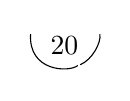
\begin{tikzpicture}[baseline=(n.base)]\node (n) at (0,0) {20};\draw (-.43,.15) .. controls (-.46,-.33) and (.06,-.34) .. (.17,-.25);\draw (.20,-.24) .. controls (.35,-.18) and (.47,.04) .. (.45,.15);\end{tikzpicture}}

Ce sont aussi les \deleted{diagr.} flèches en traits pleins du diagramme fondamental (17)

Avec l'ens ordonné $I$, fabriquons donc un \deleted{ens ordonné} \uline{diagramme} dont les sommets sont \deleted{des ``lettres'' $\unsure{x|i}\ i^*$} des symboles \deleted{$i_{**}$} $[i]$, $[i,j]$, $[i,j]^*$, où $i,j\in I$, $j$ un succ. de $i$. Les flèches du diagramme sont \unsure{des|de} trois types qui sont toutes décrites ds
\diagram{$(19)\qquad$\begin{tikzcd}[column sep=large,row sep=large]
{[i,j]^*} \arrow[r] \arrow[d] & {[i,j]} & i^* \arrow[l] \\
{[j]^*} & &
\end{tikzcd}}

Désignons par $\widetilde I$ ce diagramme, dont l'ens des sommets \deleted{s'identifie} \unsure{à|a} \deleted{$\unsure{I\times I_\Delta}$} \inserted{le cardinal} $\operatorname{card}I+2\nu$ \deleted{\unsure{card.}} \inserted{où $\nu=\operatorname{card}$} de l'ens des drapeaux $(i<j)$ ``élémentaires'' \inserted{i.e. tels que $j$ soit successeur de $i$} et le nb des flèches est $3\nu$. Si $I$ contient \unsure{ex.ctt|ex.ct} deux élts $i,j$ avec $i<j$, \inserted{i.e. $I\simeq\Delta_1$,} ce diagramme est en. (19). Si $I=\Delta_r=(0,1,\ldots,r)$, on trouve (en employant maintenant les symboles pour les $X_i^*,V_{ij}^*,V_{ij}$ qui réalisent le diagramme)

\margin{64}

\scanpage{66}
\diagram{\deleted{\begin{tikzcd}[column sep=small]
V \arrow[r] & V_{0,1} & X_0^* \arrow[l]
\end{tikzcd}}}

\margin{\uline{NB} ou mieux
\diagram{\begin{tikzcd}[row sep=small,column sep=small]
X_0^* \arrow[d] \arrow[r,dash] & {} \\
V_{01} & V_{01}^* \arrow[l] \arrow[d] \\
{} & X_1^* & {} \arrow[l]
\end{tikzcd}}}

\diagram{(20)\qquad
\begin{tikzcd}[column sep=.3em,row sep=1.2em]
X_0^* \arrow[r] & \underset{\deleted{\downarrow}}{V_{0,1}^{\unsure{*|\deleted{*}}}} & V_{0,1}^* \arrow[l] \arrow[d] & & & & & & & \\
& & X_1^* \arrow[r] & V_{1,2} & V_{1,2}^* \arrow[l] \arrow[d] & & & & & \\
& & & & X_2^* \arrow[r] & V_{2,3} & V_{2,3}^* \arrow[l] \arrow[d] & & & \\
& & & & & & X_3^* & & & \\
& & & \widetilde\Delta_n & & & \mathord{-}\;\mathord{-}\;\mathord{-}\;\mathord{-} & {} \arrow[d] & & \\
& & & & & & & X_{n-1}^* \arrow[r] & V_{n-1,n} & V_{n-1,n}^* \arrow[l] \arrow[d] \\
& & & & & & & & & X_n^*.
\end{tikzcd}}

Si $I$ est le diagramme
\diagram{\begin{tikzcd}[column sep=small,row sep=small]
& a \\
\unsure{\circ|\bullet} \arrow[ru] \arrow[rd] & \\
& b
\end{tikzcd}}, on trouve
\diagram{(21)\qquad
\begin{tikzcd}[column sep=small,row sep=large]
\deleted{\unsure{X_b^*|X_a^*}} & V_{0,b}^* \arrow[r] \arrow[d] & V_{0,b} & X_0^* \arrow[l] \arrow[r] & V_{0,a} & V_{0,a}^* \arrow[l] \arrow[d] \\
& X_b^* & & & & X_a^*.
\end{tikzcd}}

Si $I$ est le diagramme
\diagram{\begin{tikzcd}[column sep=small,row sep=small]
a\mathord\cdot \arrow[rd] & \\
& c \\
b\mathord\cdot \arrow[ru,leftrightarrow] &
\end{tikzcd}}, on trouve
\diagram{(22)\qquad
\begin{tikzcd}[column sep=large,row sep=large]
X_a^* \arrow[d] & & X_b^* \arrow[d] \\
V_{a,c} \arrow[d,leftrightarrow] & & V_{b,c} \\
V_{a,c}^* \arrow[r] & X_c^* & V_{b,c}^* \arrow[u] \arrow[l]
\end{tikzcd}},
etc.

\deleted{La première chose qu'on aimerait préciser est le} Supposons qu'on dispose sur $I$ d'une fonction à valeurs entières

\margin{65}

\scanpage{67}
\mspage{21}
\[
(23)\qquad I\xrightarrow{\underline{d}}\mathbb Z
\qquad (\text{i.e } I=\coprod_m I_m)
\]
jouant le rôle d'une fonction dimension
(on aurait une présentation en quelque sorte
duale avec une fonction type codimension),
satisfaisant la condition
\[
(24)\qquad\text{Si }i,j\in I\,\deleted{\unsure{\varnothing}},\ i\leq j,\text{ alors }d(j)=d(i)+1\Longleftrightarrow j\text{ succ. de }i
\]
Posons alors, pour $m,n_{\deleted{\unsure{2|q}}}\in\mathbb Z$
\[
(25)\qquad\left\{\begin{aligned}
X_m^*&=\coprod_{\substack{i\in I_m\\\deleted{\unsure{d(i)}}}}X_i^*\\[1.5em]
V_{m,\deleted{\unsure{n}}\inserted{m+1}}^{\deleted{\unsure{*}}}&=\coprod_{\substack{(i,j)\in I\times I\\i\leq j,\ d(i)=m\\d(j)=m+1}}V_{i,j}\\[1.5em]
V_{m,m+1}^*&=\coprod_{\substack{i,j\text{ comme}\\\text{dessus}}}V_{ij}^*
\end{aligned}\right.
\]
de sorte qu'on a les diagrammes
\diagram{\begin{tikzcd}[column sep=large,row sep=1em]
(26) & X_m^* \arrow[r] & V_{m,m+1}^{\deleted{\unsure{*}}} & V_{m,m+1}^* \arrow[l] \arrow[dd] \\
(\mathrm{Diag})_m & & & \\
& & & X_{m+1}^*
\end{tikzcd}}
s'insérant dans un diagramme commun \unsure{\inserted{\unsure{\uline{qui n'est autre que}|qui \uline{n'est autre que}} (20)}}% doubt concerns placement after commun, not the inserted words.

infini en principe, mais que nous
écrirons sous forme finie en \deleted{\unsure{présumant|privilégiant}}
simplifier \unsure{\deleted{$I$ fini}|$I$ fini}, \inserted{$\unsure{d(I)|d(I)d}$ fini et $\subset\mathbb N$)} et en n'écrivant pas les
\deleted{\unsure{composantes} \unsure{vides}} \inserted{\unsure{partie|parties} du diagramme} \unsure{correspondant,|correspondants} à : des
sommets occupés par des espaces vides :
\margin{66}

\scanpage{68}
Dans le cas d'une fonction \uline{codimension}
(\uline{$d(j)=j-1$} si $j$ succ. de $i$) on \deleted{peut} considère
des $V_{\unsure{d|g},d-1},V_{d,d-1}^*$ au lieu des $V_{d,d+1},V_{d,\unsure{d+1}}^*$,
et le diagramme prend la forme

\deleted{(27)} (Cas d'une fonction codimension)

\diagram{$(27)\qquad$
\begin{tikzcd}[column sep=.5em,row sep=1.8em]
X_n^* \arrow[r] & V_{n,n-1} & V_{n\unsure{,|+}n-1}^* \arrow[l] \arrow[d] & & & & & \\
& & X_{n-1}^* \arrow[r] & V_{n-1,n-2} & V_{n-1,n-2}^* \arrow[l] \arrow[d] & & & \\
& & & & \unsure{X_{m-1}^*|X_{n-1}^*} & & & \\
& & & & {\begin{tikzpicture}[baseline=-.5ex,x=1em,y=1em]\draw[line width=.4pt] (0,0) -- (.45,.01);\draw[line width=.4pt] (.7,.03) -- (1.5,.06) -- (1.9,.12) -- (2.1,.12);\end{tikzpicture}} & {} \arrow[d] & & \\
& & & & & X_1^* \arrow[r] & V_{1,0} & V_{1,0}^* \arrow[l] \arrow[d] \\
& & & & & & & X_0^*
\end{tikzcd}}

\margin{67}

\scanpage{69}
\mspage{22}
\uline{Th. de recollement des tubes} (\unsure{1\textsuperscript{ère}|1\textsuperscript{ière}|p\textsuperscript{re}} version) Considérons le diagramme de type $\widetilde I$, formé par les $X_i^*,V_{i,j}^*,V_{i,j}$ ($i,j\in I$, $j$ un successeur de $i$) et les trois types de flèches \unsure{y} figurant (en trait plein) ds (17). Alors $X$ s'identifie au \deleted{topos} \inserted{topos} $\underset{\longrightarrow}{\mathrm{Lim}}$ de ces topos.

\margin{Pour que cet énoncé puisse prendre un sens précis, il \unsure{faut} sans doute supp. $X$ \uline{sobre}, i.e. déterminé par $\operatorname{Top}(X)\ldots$}

\deleted{Faute de disposer de définitions en forme pour les voisinages tubulaires, je vais faire une démonstration, lorsqu'on \deleted{\unsure{pose}} $X$ remplace \deleted{\unsure{les|chaque}} $V_{ij}$ par des \inserted{vrais} vrais ouverts de $X_j$\unsure{,} de la forme $\bar V_{i,j}\setminus R_{i,j}\cap\bar V_{i,j}$, où $\bar V_{i,j}$ est un voisinage de $X_i$ dans $X_j$, et qu'on pose $\unsure{U_{ij}^*|V_{ij}^*}=U_{ij}\setminus X_i^*$. \deleted{Alors} \deleted{des \unsure{voisinages} $V_{ij}$}}

On va en donner une démonstration heuristique ci-dessous. Mais avant de le faire, je vais le généraliser, en un énoncé qui permet d'exprimer \unsure{égal\textsuperscript{t}|égalem\textsuperscript{t}} les ``topos canoniques'' associés à la \unsure{st.tific\textsuperscript{n}|st.tificat\textsuperscript{n}}, en termes du système inductif de type $\widetilde I$ formé des topos élémentaires.

\margin{68}

\scanpage{70}
\mspage{23}
\deleted{2}4. \uline{Topos canoniques associés} à \uline{une stratification
globale.}

On va montrer comment, à une situation
stratifiée donnée, on peut en associer d'autres.

A) Images inverses générales. Rappelons les
axiomes utilisés jusqu'à présent :
\[
(1)\quad\left\{\begin{aligned}
&\text{a) }X_i\text{ fermés},\ (X_i)_{i\in I}\text{ loc. \unsure{finie|fini}}\\
&\text{b) }i\leq j\Longrightarrow X_i\leq X_j\\
&\text{c) }X=\bigcup X_i\\
&\text{d) }\forall i,j\in I,\ \unsure{\text{on a}|\ldots}\quad X_i\cap X_j=\bigcup_{\uline{\unsure{h|k}}<i,j}X_k
\end{aligned}\right.
\]

Notons que pour tt $X'$ au-dessus de
$X$, la famille des
\[
(2)\qquad X'_i\overset{\mathrm{def}}=\deleted{\unsure{X'\times_X}}X_i\times_X X'
\]
satisfait les \illegible{1} $=^{\mathrm s}$ conditions.

D'ailleurs le système $\frac12$ simpl des
$X_{\Delta_r}$ \unsure{a|—} comme image inverse celui
des $X'_{\Delta_r}$, défini par les $X'_i$,
\deleted{\unsure{d}} i.e. des iso
\[
(3)\quad\left\{\begin{aligned}
X'_{\Delta_r}&\simeq X_{\Delta_r}\times_X X'\\
X'^{*}_{\Delta_r}&\simeq X^*_{\Delta_r}\times_X X'\\
\dot X'_{\Delta_r}&=\dot X_{\Delta_r}\times_X X'
\end{aligned}\right.
\]

\margin{69}

\scanpage{71}
\uline{NB} Nous appliquerons ces remarques surtout au
cas où $X'$ est un ouvert de $X$. C'est pour
pouvoir prendre de telles images inverses sans
ennui, qu'il n'aurait pas été commode
de supposer les $X_i$ ou les $X_i^*$ non vides,
ou encore que $\unsure{I|i}\mapsto X_i$ est un \uline{plong\textsuperscript{t}}
d'ens ordonnés $I\hookrightarrow\mathcal P(X)$.

Lorsque $X'\to X$ est une imm. loc\textsuperscript{le} \deleted{\unsure{p}} \inserted{propre}
\deleted{(\unsure{plus gén.}} \inserted{mais \uline{\uuline{pas}}} (ou une imm. ouverte !) alors
la formation des images inverses des
parties \deleted{\unsure{les}} fermées de $X$ commute à la
formation des voisinages tubulaires de
une telle partie dans une autre. Notons
d'ailleurs que pour $i<j$, on aura
(sans hyp. d'ailleurs que $X'-X$ soit une
imm. local)
\[
(4)\quad\left\{\begin{aligned}
R'_{ij}&=R_{ij}\times_X X'\\
S'_{ij}&=S_{ij}\times_X X'
\end{aligned}\right.,
\]
% Diagonal marginal note; the local doubts include the crowded attachment of comme.
\margin{Il y a ici une propriété formelle importante des tubes qu'il faut vérifier --- \unsure{ça est valable} pour les topos définis \unsure{comme} germes d'espaces \unsure{en dehors hyp. métriques} (p.ex. $X$ compact --- brrr!)}

d'où, en le cas d'une imm. local \inserted{propre},
des iso
\[
(5)\quad\left\{\begin{aligned}
V'^{\deleted{\unsure{*}}}_{i,j}&\simeq V_{i,j}\times_X X'\\
V'^{*}_{i,j}&\simeq V^*_{i,j}\times_X X'
\end{aligned}\right.\qquad i\leq j
\]

% Thin grey foliation at lower left, in another hand; no dark author page number observed.
\margin{70}

\scanpage{72}
\mspage{24}
et plus généralement
\[
(6)\quad V'{}^{j}_{i,\unsure{k|h}}\simeq V^{j}_{i,\unsure{k|h}}\times_X X',
\]
tant qu'à faire.

Ceci montre en particulier que la démonstration du th. de recollement, du th. énoncé p.22, est une question \uline{locale} sur $X$ \textcircled{$*$} --- ce qui permet p.ex. de nous réduire au cas où \deleted{\unsure{I}} \uline{$I$ est fini}.

\margin{\textcircled{$*$} \uuline{non}, ce n'est pas absolument clair, car les restrictions au dessus d'un ouvert ne commutent pas tt. à fait à la formation des topos élémentaires\dots C'est un panneau \unsure{dans lequel} j'ai tendance à tomber, depuis le début de mes réflexions, dans le cas des croisements normaux\dots}

\deleted{Considérons p.ex. le cas où $X'=$}

B) \uline{Cas d'un} $X_{I'}$. \deleted{Soit}

Soit $I'$ une partie de $I$ telle que
\[
(7)\quad i\leq j\in I'\quad\Longrightarrow\quad i\in I'
\]
et soit
\[
(8)\quad X_{I'}=\bigcup_{i\in I'}X_i\qquad\text{(partie fermée de $X$)}
\]
On a bien sûr
\[
(9)\quad I'\subset I''\quad\Longrightarrow\quad X_{I'}\subset X_{I''},
\]
plus gén\textsuperscript{\unsure{t|l}}.
\[
\unsure{(10)|(18)|(19)}\quad X_{I'\cup I''}=X_{I'}\cup X_{I''}
\]
plus gén.
\[
\left\{\begin{aligned}
\deleted{\bigcup_\alpha}X_{\bigcup_\alpha I'_\alpha}&=\bigcup_\alpha X_{I'_\alpha}\\
\text{aussi}\quad X_{\varnothing}&=\varnothing
\end{aligned}\right.
\]
\unsure{b|6} et aussi
\[
\unsure{(11)|(91)}\quad X_{I'\cap I''}=X_{I'}\cap X_{I''}\qquad
\left(\text{\inserted{donc} }X_{\deleted{\unsure{\varnothing}}\inserted{I}}=X\right)
\]
grâce à (11 d). Dans ces formules,

\margin{71}

\scanpage{73}
$I'$, $I''$, les $I'_\alpha$ sont des parties de $I$ satisfai-\linebreak sant (7) (des \uline{cribles} de $I$)

Si dans A) on prend $X'=X$, il est plus commode de travailler avec la stratification de $X'$ définie par les $X_i$ avec $i\in I'$ --- il est clair que les conditions (11) relatives à $X'=X_{I'}$ sont satisfaites. Les ``parties cribles'' de $X'$ pour cette stratification, \unsure{ou|—} pour celle induite au sens général des espaces au dessus de $X$, sont les $=^{\mathrm s}$ --- ce sont \inserted{donc} les traces \deleted{\unsure{inverses|induites}} \inserted{sur} $X'=X_{I'}$ des parties-cribles de l'espace stratifié $X$.

Ici, les espaces élémentaires pour la stratification de type $I'$ de \deleted{\unsure{X|\xi}} $X'=X_{\unsure{J'|I'}}$, sont les espaces
\figure{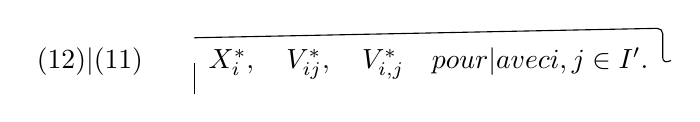
\begin{tikzpicture}
\node[inner sep=5pt] (f) {$X_i^*,\quad V_{ij}^*,\quad V_{i,j}^{\deleted{\unsure{*}}}\quad\text{\unsure{pour|avec} }i,j\in I'.$};
\node[anchor=base east] at ([xshift=-1.5em]f.base west) {$\unsure{(12)|(11)}$};
\draw[rounded corners=2pt] ([yshift=-.4ex]f.north west)--([yshift=.4ex]f.north east)--(f.east)--([xshift=.3em,yshift=.1em]f.east);
\draw (f.west)--(f.south west);
\end{tikzpicture}}

% One cancellation covers this paragraph and the following formula (13).
\deleted{Combinant les deux opérations, on a p.ex. une stratification pour tt ouvert $U'$ d'un $X'=X_{I'}$, avec les espaces \deleted{élémentaires} associés, qui sont donc les}
\[
\deleted{(13)\quad U'\cap X_i^*,\quad U'\cap V_{ij}^*,\quad U'\cap V_{ij}\qquad(i,j\in I')}
\]

\margin{72}

\scanpage{74}
\mspage{25}
\unsure{Revenons|Revenant} pour un instant à $X$, et
considérons l'ens \deleted{\unsure{de|des}} $I_0$ des $i\in I$ tel que
$X_i=\varnothing$. C'est un crible, et on a
$X_i^*=\varnothing$, $V_{ij}^*=V_{ij}=\varnothing$ si $i\in I_0$. Donc négligeant
les espaces vides, on voit que le diagramme
de type $\widetilde I$ défini par l'espace stratifié $X$
ne change pas ess\textsuperscript{t}. en remplaçant $I$ par
$I\setminus I_0$, ou plus gén par $I\setminus I'_0$, où $I'_0\subset I'$
est un crible,
ce qui donne lieu \unsure{à|:} un diagramme
$\widetilde{I\setminus I'_0}$ qui est \uline{contenu} dans $\widetilde I$ (cela est
vrai pour \uline{tt} crible de $I$).

Si p.ex. on a deux cribles
\[
(\unsure{14|16})\quad I''\subset I'\subset I
\]
d'où
\[
(15)\quad X_{I''}\subset X_{I'}\quad\text{et}\quad U_{I',I''}\overset{\mathrm{def}}{=}X_{I'}\setminus X_{I''},
\]
on peut \deleted{\unsure{sur}} (et on \unsure{va|a}) sur $U_{I',I''}$ regarder
plutôt la \deleted{filtration} \inserted{stratification} de type $I'\setminus I''$,
définie par les \deleted{$X_{i'}\setminus X_{i'}\cap X_{I''}\quad(i'\in I')\subset X$}
\[
(16)\quad X_{i',\unsure{\deleted{\unsure{X}}\inserted{I',U''}|\unsure{U|X}_{I',U''}}}=X_{i'}\setminus X_{i'}\cap X_{I''}\subset U_{I',I''}
\]
dont les topos élémentaires sont donc les
$X_{i'}^*$ $(i'\in I'\setminus I'')$ et des $V^*_{i',j'X'}$, $V_{i',j'X'}$

% Thin grey foliation at the lower left, in another hand.
\margin{73}

\scanpage{75}
associés aux couples $(i',j')$ avec $i'\in I'\setminus I''$, $j'$
successeur de $i'$, On a
\diagram{\(\displaystyle (17)\quad\left\{\vcenter{\hbox{\begin{tikzcd}[row sep=large,column sep=large]
V_{i',j'X'} \arrow[r,hook] \arrow[d,phantom,"\cup"{description}] & V_{i',j'} \arrow[d,phantom,"\cup"{description}]\\
V^*_{i',j'X'} \arrow[r,hook] & V^*_{i',j'}
\end{tikzcd}}}\right.\)}

\margin{$\Vert$}
mais il n'est pas clair en général que
ce soient \deleted{des} $\unsure{\overline{\mathrm m}}$ \inserted{\uline{seulement}} des équivalences d'homotopie\dots
Donc il faut mieux ne pas trop s'avancer
quand il s'agit de comparer les constructibles
sur un $X_{I'}$, et sur un $U_{I',I''}\unsure{=|\supset}X_{I'}\setminus\unsure{X|A}_{I''}$.

Je vais me dispenser par la suite de
\deleted{\unsure{m'étendre}} \inserted{regarder} plus \unsure{particulièrem\textsuperscript{t}|particulièrement} ce qui se
passe en s'induisant ainsi sur un ouvert
$U_{I',I''}$\dots.

C) \uline{Les} $V^{I'''}_{I',I''}$.

On suppose donné des cribles
\diagram{\begin{tikzcd}[column sep=small,row sep=small]
& I' \arrow[dr,phantom,"\subset"{description}] & &\\
(18) & & I'' \arrow[r,phantom,"\subset"{description}] & I,\\
& I''' \arrow[ur,phantom,"\subset"{description}] & &
\end{tikzcd}}
d'où
\diagram{\begin{tikzcd}[column sep=small,row sep=small]
& X_{I'} \arrow[dr,phantom,"\subset"{description}] & &\\
(19) & & X_{I''} \arrow[r,hook] & X_I=X\\
& X_{I'''} \arrow[ur,phantom,"\subset"{description}] & &
\end{tikzcd}}

\margin{74}

\cotefile{152}

\scanpage{2}
\figure{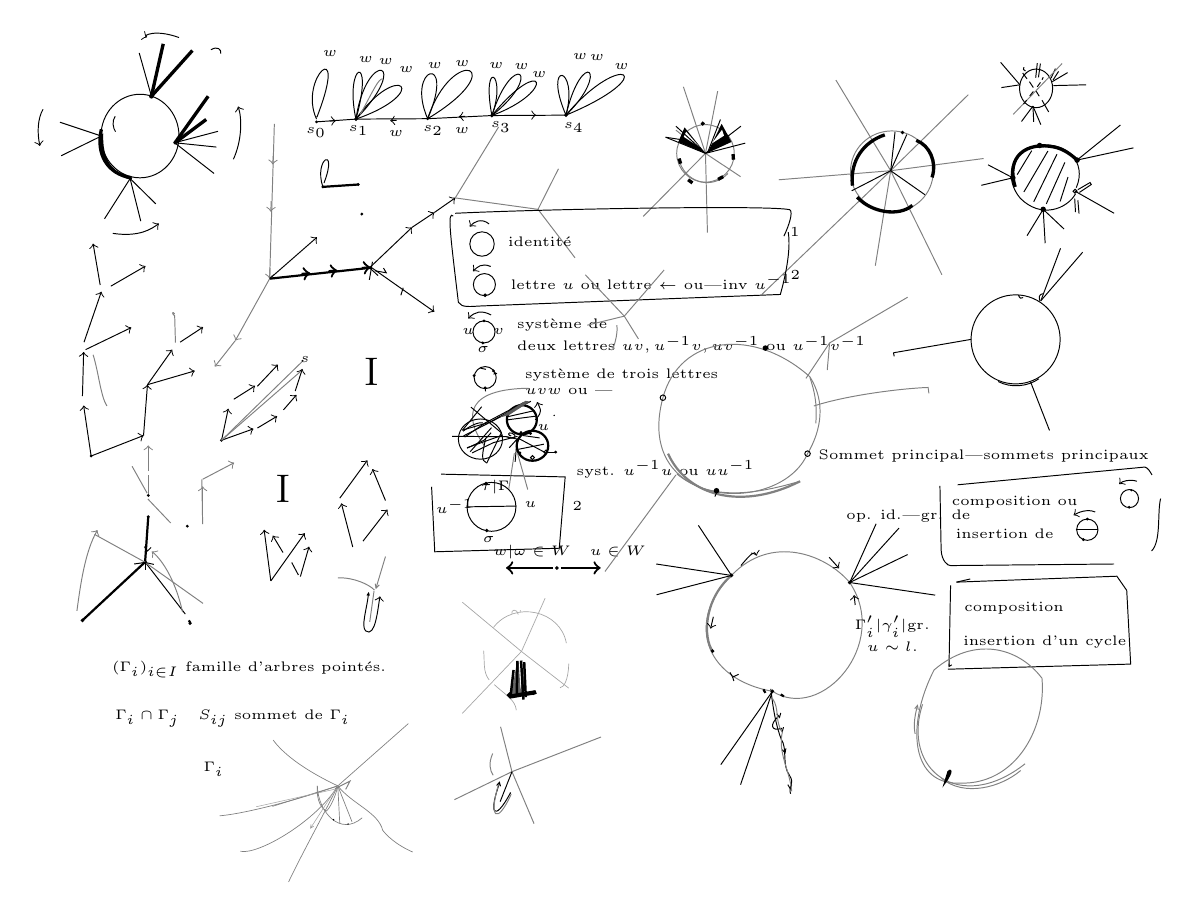
\begin{tikzpicture}[x=.005cm,y=-.005cm,line width=.35pt,every node/.style={font=\tiny,inner sep=1pt}]
\path[use as bounding box] (105,20) rectangle (2990,2218);
% G01: upper-left wheel
\draw (390,295) ellipse (99 and 106); % G01.circ
\draw[very thick] (292,278) .. controls (278,340) and (306,391) .. (368,401); % G01.over1
\draw[thick] (294,289) .. controls (291,353) and (316,392) .. (369,403); % G01.over2
\draw (327,245) .. controls (318,257) and (322,276) .. (328,284); % G01.inner
\draw[very thick] (419,194)--(449,61); % G01.top1
\draw[very thick] (419,194)--(523,78); % G01.top2
\draw (419,194)--(388,84); % G01.top3
\draw (292,295)--(187,260); % G01.left1
\draw (292,295)--(190,345); % G01.left2
\draw[very thick] (479,312)--(563,194); % G01.right1
\draw[very thick] (479,312)--(558,253); % G01.right2
\draw (478,312)--(588,283); % G01.right3
\draw (478,312)--(584,323); % G01.right4
\draw (478,312)--(578,390); % G01.right5
\draw (365,403)--(300,505); % G01.bottom1
\draw (365,403)--(392,511); % G01.bottom2
\draw (365,403)--(430,467); % G01.bottom3
\fill (419,194) circle(6); % G01.pttop
\fill (479,312) circle(5); % G01.ptright
\fill (292,295) circle(4); % G01.ptleft
\fill (365,403) circle(5); % G01.ptbottom
\draw[->] (489,45) .. controls (428,23) and (398,40) .. (408,44); % G01.rot_top
\draw[->] (144,227) .. controls (130,251) and (129,287) .. (136,320); % G01.rot_left
\draw[->] (321,542) .. controls (390,552) and (420,530) .. (438,517); % G01.rot_bottom
\draw[->] (627,354) .. controls (649,306) and (649,250) .. (639,220); % G01.rot_right
\draw (570,76) .. controls (587,66) and (597,75) .. (595,86); % G01.isolated
% G02: five-vertex loop chain
\fill (838,259) circle(4); % G02.s0_point
\fill (938,252) circle(5); % G02.s1_point
\fill (1120,251) circle(4); % G02.s2_point
\fill (1283,243) circle(5); % G02.s3_point
\fill (1471,242) circle(5); % G02.s4_point
\draw (838,259)--(938,252); % G02.edge1
\draw (1120,251)--(938,252); % G02.edge2
\draw (1283,243)--(1120,251); % G02.edge3
\draw (1283,243)--(1471,242); % G02.edge4
\draw[->] (871,257)--(887,256); % G02.head1
\draw[->] (1041,255)--(1025,256); % G02.head2
\draw[->] (1215,245)--(1199,246); % G02.head3
\draw[->] (1379,242)--(1395,242); % G02.head4
\draw (838,252) .. controls (790,147) and (923,31) .. (839,247); % G02.s0a
\draw (938,252) .. controls (907,109) and (987,78) .. (938,252); % G02.s1a
\draw (938,252) .. controls (965,71) and (1083,103) .. (938,252); % G02.s1b
\draw (938,252) .. controls (1048,99) and (1133,184) .. (938,252); % G02.s1c
\draw (1120,251) .. controls (1062,118) and (1194,80) .. (1120,251); % G02.s2a
\draw (1120,251) .. controls (1184,58) and (1339,119) .. (1120,251); % G02.s2b
\draw (1283,243) .. controls (1255,94) and (1323,134) .. (1283,243); % G02.s3a
\draw (1283,243) .. controls (1336,74) and (1419,135) .. (1283,243); % G02.s3b
\draw (1283,243) .. controls (1416,81) and (1451,181) .. (1283,243); % G02.s3c
\draw (1471,242) .. controls (1410,100) and (1505,115) .. (1471,242); % G02.s4a
\draw (1471,242) .. controls (1512,68) and (1587,128) .. (1471,242); % G02.s4b
\draw (1471,242) .. controls (1613,73) and (1718,139) .. (1471,242); % G02.s4c
\node at (872,85) {$w$}; % G02.w01
\node at (963,102) {$w$}; % G02.w02
\node at (1014,107) {$w$}; % G02.w03
\node at (1066,125) {$w$}; % G02.w04
\node at (1138,115) {$w$}; % G02.w05
\node at (1208,111) {$w$}; % G02.w06
\node at (1294,116) {$w$}; % G02.w07
\node at (1358,118) {$w$}; % G02.w08
\node at (1403,140) {$w$}; % G02.w09
\node at (1507,92) {$w$}; % G02.w10
\node at (1550,95) {$w$}; % G02.w11
\node at (1612,118) {$w$}; % G02.w12
\node at (1040,289) {$w$}; % G02.w13
\node at (1207,282) {$w$}; % G02.w14
\node at (837,286) {$s_{0}$}; % G02.s0_label
\node at (945,282) {$s_{1}$}; % G02.s1_label
\node at (1134,281) {$s_{2}$}; % G02.s2_label
\node at (1306,272) {$s_{3}$}; % G02.s3_label
\node at (1491,273) {$s_{4}$}; % G02.s4_label
\draw[gray] (949,240) .. controls (980,184) and (995,148) .. (1006,150); % G02.faint_return01
% G03: small loop and edge with isolated point
\draw (854,424) .. controls (830,351) and (894,318) .. (857,414); % G03.loop
\draw[thick] (854,424)--(944,418); % G03.edge
\fill (854,424) circle(4); % G03.junction
\fill (944,418) circle(4); % G03.right
\fill (953,493) circle(4); % G03.isolated
% G04: pale wheel with dark sectors
\draw[gray] (1769,170)--(1825,339); % G04.pencil1
\draw[gray] (1825,339)--(1830,540); % G04.pencil2
\draw[gray] (1856,181)--(1825,339); % G04.pencil3
\draw[gray] (1825,339)--(1667,499); % G04.pencil4
\draw[gray] (1825,339)--(1750,280); % G04.pencil5
\draw[gray] (1825,339)--(1914,398); % G04.pencil6
\draw[gray] (1825,339) ellipse (73 and 73); % G04.circ
\draw[gray] (1760,363) .. controls (1781,418) and (1845,429) .. (1882,390); % G04.over
\draw[very thick] (1815,261)--(1821,266); % G04.tick1
\draw[very thick] (1758,352)--(1762,365); % G04.tick2
\draw[very thick] (1781,406)--(1792,414); % G04.tick3
\draw[very thick] (1857,405)--(1870,398); % G04.tick4
\draw[very thick] (1895,341)--(1896,355); % G04.tick5
\fill (1825,339)--(1772,273)--(1756,310)--cycle; % G04.sectorL
\fill[white] (1810,323)--(1776,284)--(1770,297)--cycle; % G04.gapL
\fill (1830,338)--(1866,264)--(1891,310)--cycle; % G04.sectorR
\fill[white] (1841,314)--(1867,279)--(1872,294)--cycle; % G04.gapR
\draw (1825,339)--(1724,298); % G04.ink1
\draw (1724,298)--(1775,306); % G04.ink2
\draw (1825,339)--(1750,270); % G04.ink3
\draw (1830,338)--(1863,253); % G04.ink4
\draw (1825,339)--(1915,270); % G04.ink5
\draw (1825,339)--(1926,313); % G04.ink6
% G05: three-arc wheel
\draw[gray] (2295,383)--(2156,153); % G05.pencil1
\draw[gray] (2295,383)--(2492,190); % G05.pencil2
\draw[gray] (2295,383)--(2531,352); % G05.pencil3
\draw[gray] (2295,383)--(2425,647); % G05.pencil4
\draw[gray] (2295,383)--(2256,624); % G05.pencil5
\draw[gray] (2295,383)--(1968,697); % G05.pencil6
\draw[gray] (2295,383)--(2011,406); % G05.pencil7
\draw[gray] (2298,385) ellipse (105 and 103); % G05.pale_circ
\draw[very thick] (2198,421) .. controls (2191,356) and (2228,309) .. (2280,292); % G05.arc1
\draw[very thick] (2360,306) .. controls (2394,319) and (2413,360) .. (2400,400); % G05.arc2
\draw[very thick] (2210,450) .. controls (2247,490) and (2316,500) .. (2350,471); % G05.arc3
\fill (2396,340) circle(3); % G05.arc_return
\draw (2295,383)--(2196,434); % G05.ink1
\draw (2295,383)--(2382,444); % G05.ink2
\draw (2295,383)--(2306,285); % G05.ink3
\draw (2295,383)--(2336,291); % G05.ink4
\fill (2325,286) circle(5); % G05.topdot
% G06: small ray circle at top right
\draw (2664,174) ellipse (42 and 49); % G06.circ
\draw (2623,165)--(2574,108); % G06.ray1
\draw (2623,165)--(2576,172); % G06.ray2
\draw (2705,157)--(2744,134); % G06.ray3
\draw (2708,167)--(2791,165); % G06.ray4
\draw (2656,219)--(2627,258); % G06.ray5
\draw (2656,219)--(2676,266); % G06.ray6
\draw (2656,219)--(2658,259); % G06.ray7
\draw (2663,147)--(2667,110); % G06.tick1
\draw (2670,146)--(2675,111); % G06.tick2
\draw (2702,148)--(2713,124); % G06.tick3
\draw (2707,153)--(2721,131); % G06.tick4
\draw[gray] (2606,240)--(2730,111); % G06.faint_diag
\draw (2630,135)--(2641,150); % G06.fragment1
\draw (2647,157)--(2657,172); % G06.fragment2
\draw (2664,181)--(2672,194); % G06.fragment3
\draw (2679,204)--(2696,234); % G06.fragment4
\draw (2632,214)--(2640,204); % G06.fragment5
\draw (2648,193)--(2657,182); % G06.fragment6
\draw (2667,170)--(2675,159); % G06.fragment7
\draw (2679,152)--(2682,146); % G06.fragment8
\draw (2633,120) .. controls (2630,125) and (2632,128) .. (2637,130); % G06.tiny_curl
% G07: hatched five-mark disc
\draw (2766,426) .. controls (2794,361) and (2741,309) .. (2673,319) .. controls (2593,330) and (2584,407) .. (2624,453) .. controls (2677,506) and (2742,480) .. (2764,442); % G07.circ
\draw[very thick] (2611,424) .. controls (2586,346) and (2640,308) .. (2711,323) .. controls (2734,328) and (2753,342) .. (2768,356); % G07.over
\fill (2605,401) circle(7); % G07.pt_left
\fill (2673,319) circle(7); % G07.pt_top
\fill (2768,356) circle(7); % G07.pt_upperright
\fill (2682,481) circle(7); % G07.pt_bottom
\draw (2763,435) circle(5); % G07.ring
\draw (2605,401)--(2542,368); % G07.left1
\draw (2605,401)--(2525,420); % G07.left2
\draw (2768,356)--(2878,267); % G07.rightup1
\draw (2768,356)--(2911,325); % G07.rightup2
\draw (2770,431)--(2801,413)--(2804,418)--(2774,438); % G07.short1
\draw (2763,435)--(2862,491); % G07.longright
\draw (2682,481)--(2641,548); % G07.bottom1
\draw (2682,481)--(2687,567); % G07.bottom2
\draw (2682,481)--(2735,531); % G07.bottom3
\draw (2762,454)--(2764,488); % G07.tick1
\draw (2770,458)--(2773,492); % G07.tick2
\draw (2616,393)--(2653,332); % G07.hatch1
\draw (2633,437)--(2694,333); % G07.hatch2
\draw (2658,462)--(2717,341); % G07.hatch3
\draw (2690,467)--(2737,362); % G07.hatch4
\draw (2725,461)--(2745,399); % G07.hatch5
% G08: large unmarked circle
\draw (2612,811) ellipse (113 and 113); % G08.circ
\draw (2499,811)--(2302,845); % G08.left
\draw (2676,713)--(2726,580); % G08.upper1
\draw (2676,713)--(2782,590); % G08.upper2
\draw (2650,919)--(2698,1042); % G08.lower
\draw (2302,845)--(2304,854); % G08.left_hook
\draw (2674,714) .. controls (2670,703) and (2672,697) .. (2681,695); % G08.upper_hook
\draw (2619,698) .. controls (2622,707) and (2627,709) .. (2631,705); % G08.top_return
\draw (2568,918) .. controls (2600,935) and (2643,931) .. (2671,911); % G08.bottom_return
% G09: main pencil arrow tree
\draw[gray] (731,264)--(719,657); % G09.vertical
\draw[gray,->] (728,346)--(727,367); % G09.vert_head1
\draw[gray,->] (723,460)--(722,487); % G09.vert_head2
\draw[gray,->] (720,631)--(719,657); % G09.vert_head3
\draw[thick] (719,657)--(978,629); % G09.horizontal
\draw[thick,->] (800,645)--(822,643); % G09.hor_head1
\draw[thick,->] (869,638)--(891,636); % G09.hor_head2
\draw[thick,->] (953,630)--(975,628); % G09.hor_head3
\draw[->] (719,657)--(839,552); % G09.shortNE
\draw[gray,->] (719,657)--(632,814); % G09.SW1
\draw[gray,->] (632,814)--(580,880); % G09.SW2
\draw[->] (975,627)--(1080,527); % G09.NE1
\draw[->] (1080,527)--(1137,489); % G09.NE2
\draw[->] (1137,489)--(1190,452); % G09.NE3
\draw[gray] (1190,452)--(1300,272); % G09.NE_cont
\draw[->] (975,627)--(1137,741); % G09.SE1
\draw (1058,680)--(1052,699); % G09.SE2
\draw (956,614)--(994,649); % G09.cross1
\draw (980,614)--(972,660); % G09.cross2
\draw (987,637)--(1015,642)--(1008,630); % G09.right_return
\draw[gray] (1190,452)--(1400,481); % G09.fork_join
\draw[gray] (1400,481)--(1452,378); % G09.fork_up
\draw[gray] (1400,481)--(1494,604); % G09.fork_down
% G10: upright left arrow construction
\draw[->] (266,1107)--(247,979); % G10.a1
\draw[->] (244,955)--(247,843); % G10.a2
\draw[->] (248,818)--(292,690); % G10.a3
\draw[->] (289,673)--(271,568); % G10.a4
\draw[->] (266,1107)--(399,1055); % G10.r1
\draw[->] (252,837)--(368,781); % G10.r2
\draw[->] (316,676)--(404,625); % G10.r3
\draw[->] (399,1055)--(409,926); % G10.b1
\draw[->] (409,926)--(472,837); % G10.b2
\draw[->] (409,926)--(529,891); % G10.b3
\draw[->] (492,818)--(550,780); % G10.topside
\fill (266,1107) circle(4); % G10.root
\draw[gray] (480,819)--(478,751) .. controls (470,746) and (472,739) .. (478,746); % G10.upper_curl
\draw[gray] (271,850) .. controls (285,894) and (290,955) .. (306,980); % G10.faint_curve
% G11: small right arrow construction
% M1088: the terminal reading is open between a letter and the connected graphical curl/endpoint.
\fill (597,1067) circle(4); % G11.root
\draw[->] (597,1067)--(614,987); % G11.arrow1
\draw[->] (597,1067)--(678,1038); % G11.arrow2
\draw[->] (628,963)--(682,929); % G11.arrow3
\draw[->] (688,930)--(740,875); % G11.arrow4
\draw[->] (784,942)--(802,886); % G11.arrow6
\draw[->] (754,990)--(787,952); % G11.arrow7
\draw[->] (688,1036)--(738,1006); % G11.arrow8
\draw[gray] (597,1067)--(805,864); % G11.diag1
\draw[gray] (597,1067)--(798,892); % G11.diag2
\node at (808,862) {$\unsure{s}$}; % G11.terminal
% G12: upper isolated I
\node at (977,893) {\Large $\mathrm I$}; % G12.glyph
% G13: lower isolated I
\node at (753,1191) {\Large $\mathrm I$}; % G13.glyph
% G14: lower-left branching construction
\fill (411,1207) circle(4); % G14.upper
\fill (510,1285) circle(4); % G14.side
\fill (244,1524) circle(5); % G14.lowleft
\fill (403,1376) circle(5); % G14.centre
\fill (411,1261) circle(4); % G14.upperY
\draw[gray] (411,1203)--(411,1154); % G14.incoming1
\draw[gray,->] (411,1145)--(411,1080); % G14.incoming2
\draw[gray] (370,1133)--(408,1201); % G14.slant
\draw[gray] (410,1216)--(468,1277); % G14.slant_down
\draw[gray] (547,1166)--(549,1280); % G14.right_vertical
\draw[gray,->] (549,1280)--(549,1184); % G14.right_up
\draw[gray,->] (549,1166)--(629,1124); % G14.right_branch
\draw[thick] (244,1524)--(403,1376); % G14.main_left
\draw[thick] (403,1376)--(411,1261); % G14.main_vertical
\draw (401,1337)--(409,1348)--(418,1339); % G14.vertical_return
\draw (403,1376)--(505,1508); % G14.main_right
\draw[gray,->] (230,1500) .. controls (239,1432) and (251,1349) .. (282,1295); % G14.aux1
\draw[gray] (275,1306)--(402,1376); % G14.aux2
\draw[gray] (402,1376)--(550,1481); % G14.aux3
\draw[gray,->] (498,1503) .. controls (482,1430) and (451,1375) .. (420,1349); % G14.aux4
\draw[thick] (514,1524)--(518,1531)--(515,1534); % G14.isolated_mark
\draw (375,1381)--(403,1377)--(425,1382); % G14.central_stubs01
\draw (403,1377)--(403,1397); % G14.central_stubs02
% G15: W-shaped four-arrow construction
\draw[->] (722,1424)--(705,1294); % G15.arrow1
\draw[->] (722,1424)--(808,1303); % G15.arrow2
\draw[->] (797,1413)--(819,1337); % G15.arrow3
\draw (792,1409)--(775,1377); % G15.arrow4_1
\draw[->] (753,1352)--(727,1309); % G15.arrow4_2
% G16: four-arrow diamond
\draw[->] (897,1214)--(967,1118); % G16.arrow1
\draw[->] (1013,1220)--(980,1140); % G16.arrow2
\draw[->] (930,1338)--(901,1227); % G16.arrow3
\draw[->] (956,1323)--(1018,1243); % G16.arrow4
% G17: bent line with hairpin arrow
\draw[gray] (892,1416) .. controls (934,1415) and (971,1433) .. (985,1447); % G17.diagonal
\draw[gray] (1013,1362)--(989,1442); % G17.upright
\draw[gray] (997,1434)--(989,1442)--(987,1431); % G17.downhead_1
\draw[gray] (984,1449)--(973,1528); % G17.downhead_2
\draw[->] (970,1455) .. controls (966,1495) and (950,1540) .. (963,1551) .. controls (987,1568) and (993,1499) .. (999,1463); % G17.hairpin_1
\draw (966,1461)--(970,1455)--(972,1461); % G17.hairpin_2
% G18: first framed examples
\draw (1190,491) .. controls (1420,480) and (1990,470) .. (2039,482) .. controls (2048,488) and (2037,522) .. (2024,549); % G18.frame_1
\draw (1185,498) .. controls (1170,485) and (1176,534) .. (1198,717) .. controls (1207,732) and (1230,727) .. (1260,726)--(2015,697) .. controls (2025,661) and (2043,588) .. (2035,539); % G18.frame_2
\draw (1258,569) ellipse (31 and 31); % G18.circle1
\draw[->] (1276,518) .. controls (1256,502) and (1237,513) .. (1227,525); % G18.arrow1
\node[anchor=west] at (1316,563) {identité}; % G18.line1
\node at (2052,539) {$1$}; % G18.number1
\draw (1264,672) ellipse (28 and 28); % G18.circle2
\fill (1266,699) circle(5); % G18.bottom2
\draw[->] (1280,626) .. controls (1256,616) and (1246,628) .. (1235,638); % G18.arrow2
\node[anchor=west] at (1323,665) {lettre $u$ ou lettre \unsure{$\leftarrow$ ou|inv} $u^{-1}$}; % G18.line2
\node at (2053,649) {$2$}; % G18.number2
% G19: two-letter circle and caption
\draw (1263,792) ellipse (28 and 28); % G19.circle
\fill (1263,764) circle(4); % G19.top
\fill (1260,820) circle(4); % G19.bottom
\draw[->] (1281,749) .. controls (1256,736) and (1240,741) .. (1223,758); % G19.arrow
\node at (1223,790) {$u$}; % G19.u
\node at (1301,790) {$v$}; % G19.v
\node at (1261,836) {$\sigma$}; % G19.sigma
\node[anchor=west] at (1339,775) {système de}; % G19.line1
\node[anchor=west] at (1339,825) {deux lettres $uv,u^{-1}v,uv^{-1}$ ou $u^{-1}v^{-1}$}; % G19.line2
% G20: three-letter circle and caption
\draw (1266,908) ellipse (28 and 28); % G20.circle
\fill (1238,903) circle(4); % G20.left
\fill (1287,891) circle(4); % G20.upperright
\fill (1266,934) circle(4); % G20.bottom
\draw (1266,934)--(1267,943); % G20.bottom_stem
\node[anchor=west] at (1359,901) {système de trois lettres}; % G20.line1
\node[anchor=west] at (1359,943) {$uvw$ ou \unsure{---}}; % G20.line2
\draw (1254,884)--(1268,887); % G20.rim_return01
\draw (1288,900)--(1290,896)--(1296,898); % G20.rim_return02
% G35: pencil crossing behind central captions
\draw[gray] (1619,752)--(1520,647); % G35.NW
\draw[gray] (1619,752)--(1720,635); % G35.NE
\draw[gray] (1619,752)--(1525,775); % G35.SW
\draw[gray] (1619,752)--(1655,810); % G35.S
\draw[gray] (1600,775) .. controls (1603,792) and (1596,820) .. (1590,835); % G35.detached
% G21: three crowded and crossed circles
% Crossing/cancellation strokes are individually reproduced; no lexical deletion or replacement is inferred.
\draw[gray] (1375,935) .. controls (1190,938) and (1227,1030) .. (1264,1081); % G21.pale_left
\draw (1254,1064) ellipse (56 and 51); % G21.left_circle
\draw[thick] (1359,1015) ellipse (38 and 37); % G21.upper_circle
\draw[thick] (1386,1081) ellipse (40 and 38); % G21.lower_circle
\draw (1324,1015)--(1393,1006); % G21.upper_chord1
\draw (1324,1007)--(1390,992); % G21.upper_chord2
\draw (1352,1063)--(1416,1097); % G21.lower_chord1
\draw (1350,1090)--(1415,1077); % G21.lower_chord2
\draw (1362,1055)--(1404,1061); % G21.lower_chord3
\fill (1357,1047) circle(4); % G21.upper_bottom
\fill (1354,1099) circle(4); % G21.lower_left
\fill (1381,1050) circle(4); % G21.lower_top
\fill (1445,1097) circle(4); % G21.stem_end
\draw (1386,1111) circle(5); % G21.lower_bottom_ring
\draw (1420,1097) circle(5); % G21.lower_right_ring
\draw (1425,1097)--(1445,1097); % G21.right_stem
\node at (1414,1035) {$u$}; % G21.u
\draw[->] (1393,1015) .. controls (1417,993) and (1401,979) .. (1398,970); % G21.arrow
\draw (1214,1059)--(1266,1023)--(1364,971); % G21.crossing01
\draw (1208,1042)--(1257,982); % G21.crossing02
\draw (1211,1056)--(1382,968); % G21.crossing03
\draw (1220,1086)--(1310,1054); % G21.crossing04
\draw (1230,983)--(1307,1048)--(1270,1125); % G21.crossing05
\draw (1228,1096)--(1282,1035); % G21.crossing06
\draw (1182,1057)--(1320,1058)--(1352,1065); % G21.crossing07
\draw (1209,1041)--(1278,1021)--(1373,968); % G21.crossing08
\draw (1220,1087)--(1263,1067)--(1281,1048); % G21.crossing09
\draw (1233,1099)--(1287,1073)--(1348,1057); % G21.crossing10
\draw (1210,1044) .. controls (1225,1032) and (1248,1020) .. (1260,1023); % G21.crossing11
\draw (1267,1063) .. controls (1258,1105) and (1255,1118) .. (1270,1125); % G21.crossing12
\fill[black!65] (1302,1009)--(1368,967)--(1379,969)--(1325,1004)--cycle; % G21.crossing13
\draw (1327,1086)--(1347,1064)--(1342,1122); % G21.crossing14
\fill (1441,1004) circle(2); % G21.crossing15
\draw (1320,1058) .. controls (1344,1068) and (1348,1054) .. (1334,1049) .. controls (1323,1045) and (1323,1056) .. (1332,1056); % G21.crossing16
% G22: framed diameter circle and double arrow
\draw (1130,1185)--(1138,1350)--(1454,1341)--(1469,1160)--(1154,1153); % G22.frame
\draw (1282,1236) ellipse (62 and 62); % G22.circle
\draw (1219,1236)--(1345,1234); % G22.diameter
\fill (1268,1177) circle(5); % G22.top
\fill (1270,1296) circle(5); % G22.bottom
\node at (1291,1186) {$\unsure{\tau|\Gamma}$}; % G22.tau
\node at (1275,1318) {$\sigma$}; % G22.sigma
\node at (1381,1230) {$u$}; % G22.u
\node at (1189,1235) {$u^{-1}$}; % G22.uinv
\node at (1500,1234) {$2$}; % G22.number
\node[anchor=west] at (1490,1140) {syst. $u^{-1}u$ ou $uu^{-1}$}; % G22.line1
\node at (1480,1350) {$\unsure{w|\omega}\in W\quad u\in W$}; % G22.line2
\draw[thick,->] (1438,1391)--(1319,1391); % G22.left_arrow
\draw[thick,->] (1458,1391)--(1559,1391); % G22.right_arrow
\fill (1448,1391) circle(5); % G22.middle
\draw[gray] (1340,1100)--(1326,1190); % G22.pale_extension01
\draw[gray] (1348,1100)--(1374,1192); % G22.pale_extension02
% G23: principal pale circle
\draw[gray] (1717,959) .. controls (1760,800) and (1948,779) .. (2090,906) .. controls (2130,969) and (2120,1040) .. (2084,1101) .. controls (2015,1260) and (1640,1245) .. (1717,959); % G23.outline
\draw[gray,thick] (1730,1101) .. controls (1780,1211) and (1920,1245) .. (2065,1171); % G23.lower_over1
\draw[gray] (1752,1152) .. controls (1837,1223) and (1952,1204) .. (2065,1171); % G23.lower_over2
\draw[gray] (2080,910)--(2140,820)--(2338,704); % G23.upper_departure
\draw[gray] (2100,980) .. controls (2190,951) and (2330,935) .. (2390,933)--(2392,948); % G23.right_departure
\draw[gray] (2090,908) .. controls (2108,959) and (2107,994) .. (2105,1024); % G23.right_parallel
\draw[gray] (1750,1155)--(1570,1400); % G23.southwest
\draw (1717,959) circle(7); % G23.left
\fill (1977,833) circle(7); % G23.top
\draw (2084,1101) circle(7); % G23.right
\fill (1853,1195) circle(7); % G23.bottom
\draw (1853,1200)--(1849,1210); % G23.bottom_tick
\node[anchor=west] at (2104,1108) {\unsure{Sommet principal|sommets principaux}}; % G23.caption
\draw[gray] (2140,820)--(2134,889); % G23.upper_branch01
% G24: lower four-vertex circle
% The op. id. underline overlaps the upper slanted fan ray. The side glyph and relation remain doubtful.
\draw[gray] (1891,1410) .. controls (1777,1520) and (1816,1672) .. (1995,1704) .. controls (2120,1784) and (2295,1583) .. (2191,1428) .. controls (2129,1355) and (1991,1305) .. (1891,1410); % G24.outline
\draw[gray,thick] (1891,1410) .. controls (1820,1471) and (1819,1568) .. (1843,1602); % G24.left_over
\fill (1891,1410) circle(5); % G24.A
\fill (2191,1428) circle(5); % G24.B
\fill (1995,1704) circle(5); % G24.C
\fill (1843,1602) circle(5); % G24.D
\draw (1891,1410)--(1700,1381); % G24.A1
\draw (1891,1410)--(1701,1459); % G24.A2
\draw (1891,1410)--(1807,1283); % G24.A3
\draw (2191,1428)--(2258,1279); % G24.B1
\draw (2191,1428)--(2316,1290); % G24.B2
\draw (2191,1428)--(2338,1357); % G24.B3
\draw (2191,1428)--(2408,1460); % G24.B4
\draw (1995,1704)--(1864,1890); % G24.C1
\draw (1995,1704)--(1914,1941); % G24.C2
\draw[->] (1915,1385) .. controls (1940,1355) and (1950,1346) .. (1955,1360); % G24.headA
\draw[->] (2139,1364)--(2164,1392); % G24.headtop
\draw[->] (1845,1515)--(1838,1545); % G24.headleft
\draw (1887,1656)--(1894,1668)--(1909,1661); % G24.headlowerleft_1
\draw (1894,1668)--(1897,1678); % G24.headlowerleft_2
\draw[->] (2205,1485)--(2202,1460); % G24.headright
\draw[thick] (1972,1699)--(1977,1708); % G24.bottommarkL
\draw[thick] (2016,1712)--(2024,1717); % G24.bottommarkR
\node at (2340,1260) {\uline{\unsure{op. id.|gr. de}}}; % G24.opid
\node at (2300,1540) {$\unsure{\Gamma'_i|\gamma'_i|\mathrm{gr.}}$}; % G24.Gamma
\node at (2300,1590) {$\unsure{u\sim l}.$}; % G24.relation
\draw (1991,1698) .. controls (1997,1758) and (2007,1799) .. (2017,1825) .. controls (2034,1850) and (2018,1890) .. (2038,1917) .. controls (2053,1940) and (2034,1946) .. (2041,1964); % G24.lower_stem01
\draw (2016,1759)--(2013,1770)--(2006,1761); % G24.lower_stem02
\draw (2023,1795)--(2020,1806)--(2013,1797); % G24.lower_stem03
\draw (2029,1849)--(2027,1860)--(2019,1852); % G24.lower_stem04
\draw (2044,1941)--(2040,1951)--(2034,1941); % G24.lower_stem05
\draw (2010,1768) .. controls (1988,1787) and (1990,1807) .. (2019,1798); % G24.lower_stem06
\draw[gray] (1995,1722) .. controls (2014,1750) and (2000,1778) .. (2020,1808) .. controls (2008,1860) and (2039,1905) .. (2044,1958); % G24.lower_stem07
% G25: upper right composition/insertion frame
\draw (2420,1183)--(2423,1345) .. controls (2424,1373) and (2440,1386) .. (2447,1385)--(2862,1381); % G25.frame_leftbottom
\draw (2465,1180)--(2940,1135) .. controls (2948,1137) and (2953,1146) .. (2958,1155); % G25.frame_upper
\draw (2980,1215) .. controls (2971,1250) and (2982,1323) .. (2957,1348); % G25.frame_right
\node[anchor=west] at (2442,1223) {\uline{composition} ou}; % G25.line1
\draw (2901,1215) ellipse (23 and 23); % G25.circle1
\fill (2900,1237) circle(4); % G25.bottom1
\draw[->] (2920,1171) .. controls (2901,1165) and (2883,1171) .. (2875,1178); % G25.arrow1
\node[anchor=west] at (2452,1305) {\uline{insertion} de}; % G25.line2
\draw (2794,1294) ellipse (27 and 27); % G25.circle2
\draw (2764,1294)--(2821,1294); % G25.diameter
\fill (2794,1267) circle(4); % G25.top2
\fill (2784,1319) circle(4); % G25.bottom2
\draw[->] (2814,1249) .. controls (2793,1240) and (2770,1251) .. (2759,1257); % G25.arrow2
\fill (2906,1194) circle(3); % G25.upper_mark01
% G26: lower right composition/insertion frame
\draw (2447,1435)--(2443,1641) (2440,1648)--(2904,1635)--(2894,1448)--(2869,1412)--(2462,1427); % G26.frame
\draw (2443,1634)--(2443,1641)--(2450,1637); % G26.left_return
\draw (2462,1427)--(2497,1419); % G26.top_return
\node[anchor=west] at (2474,1492) {composition}; % G26.line1
\node[anchor=west] at (2471,1579) {insertion d'un cycle}; % G26.line2
% G27: pale oval below right frame
\draw[gray] (2405,1650) .. controls (2332,1793) and (2348,1944) .. (2472,1937) .. controls (2606,1941) and (2690,1807) .. (2679,1671); % G27.oval
\draw[gray] (2405,1650) .. controls (2505,1564) and (2618,1590) .. (2679,1671); % G27.top_arc
\draw[gray] (2376,1737) .. controls (2321,1903) and (2471,2018) .. (2636,1888); % G27.lower_return1
\draw[gray] (2424,1925) .. controls (2481,1972) and (2573,1949) .. (2625,1905); % G27.lower_return2
\draw[thick] (2442,1907) .. controls (2454,1900) and (2439,1927) .. (2434,1933)--(2442,1907); % G27.dark_mark
\draw[gray] (2357,1812) .. controls (2352,1788) and (2357,1763) .. (2363,1740); % G27.outer_return01
\draw[gray] (2356,1748)--(2363,1740)--(2365,1751); % G27.outer_return02
% G28: family-of-trees line
% Final dot after pointés is uncertain; a small terminal hook is visible.
\node[anchor=west] at (311,1649) {$(\Gamma_i)_{i\in I}$ famille d'arbres pointés\unsure{.}}; % G28.line
% G29: intersection and summit line
\node[anchor=west] at (319,1773) {$\Gamma_i\cap\Gamma_j\quad S_{ij}$ sommet de $\Gamma_i$}; % G29.line
% G30: bottom-left pencil fan
\draw[black!50,line width=.25pt] (728,1828) .. controls (766,1879) and (843,1921) .. (892,1944); % G30.audit01
\draw[black!50,line width=.25pt] (892,1944) -- (1071,1786); % G30.audit02
\draw[black!50,line width=.25pt] (892,1944) .. controls (928,1990) and (995,2011) .. (1006,2057) .. controls (1026,2082) and (1055,2100) .. (1082,2112); % G30.audit03
\draw[black!50,line width=.25pt] (892,1944) .. controls (838,2033) and (690,2120) .. (645,2110); % G30.audit04
\draw[black!50,line width=.25pt] (892,1944) .. controls (860,2010) and (799,2120) .. (767,2188); % G30.audit05
\draw[black!50,line width=.25pt] (892,1944) .. controls (810,1973) and (664,2014) .. (592,2020); % G30.audit06
\draw[black!50,line width=.25pt] (892,1944) -- (726,1996); % G30.audit07
\draw[black!35,line width=.2pt] (891,1951) -- (685,1997); % G30.audit08
\draw[black!50,line width=.25pt] (892,1944) -- (897,2040); % G30.audit09
\draw[black!50,line width=.25pt] (892,1944) -- (928,2035); % G30.audit10
\draw[black!50,line width=.25pt] (840,1944) .. controls (837,1985) and (853,2003) .. (863,2008) .. controls (877,1995) and (889,1960) .. (892,1944); % G30.audit11
\draw[black!50,line width=.25pt] (840,1944) .. controls (842,2012) and (899,2073) .. (954,2025); % G30.audit12
\draw[black!35,line width=.2pt] (892,1944) -- (823,2051); % G30.audit13
\draw[black!40,line width=.25pt] (830.691,2046.43) -- (823,2051) -- (823.961,2042.11); % G30.audit14
\fill[black] (881,2030) circle [radius=2]; % G30.audit15
\fill[black] (918,2041) circle [radius=2]; % G30.audit16
\node[anchor=center] at (577,1902) {$\Gamma_i$}; % G30.audit17
\draw[gray] (885,1951)--(923,1932)--(912,1953); % G30.NE_return01
% G31: pale crossing with dark wedge on bar
\draw[black!35,line width=.25pt] (1287,1542) .. controls (1340,1473) and (1457,1498) .. (1472,1582); % G31.audit01
\draw[black!35,line width=.25pt] (1478,1634) .. controls (1477,1675) and (1466,1694) .. (1456,1695); % G31.audit02
\draw[black!35,line width=.25pt] (1262,1601) .. controls (1265,1630) and (1260,1655) .. (1276,1675); % G31.audit03
\draw[black!35,line width=.25pt] (1289,1687) .. controls (1321,1716) and (1342,1726) .. (1345,1752); % G31.audit04
\draw[black!35,line width=.25pt] (1208,1478) -- (1358,1603) -- (1478,1696); % G31.audit05
\draw[black!35,line width=.25pt] (1418,1468) -- (1358,1603) -- (1208,1760); % G31.audit06
\draw[black!35,line width=.25pt] (1334,1507) .. controls (1330,1497) and (1347,1493) .. (1350,1509); % G31.audit07
\fill[black] (1355,1500) circle [radius=1]; % G31.audit08
\fill[black!60] (1347,1627) -- (1332,1714) -- (1365,1714) -- (1363,1632) -- (1356,1704) -- (1351,1630) -- cycle; % G31.audit09
\draw[line width=.9pt] (1348,1627) -- (1346,1715); % G31.audit10
\draw[line width=.9pt] (1357,1626) -- (1363,1725); % G31.audit11
\draw[line width=.9pt] (1365,1630) -- (1369,1719); % G31.audit12
\draw[line width=.9pt] (1338,1650) -- (1330,1720); % G31.audit13
\draw[line width=1.5pt] (1324,1710) -- (1331,1717) -- (1390,1707) -- (1392,1712); % G31.audit14
% G32: bottom crossed rays and hairpin
\draw[gray] (1334,1908)--(1305,1794); % G32.NW
\draw[gray] (1334,1908)--(1188,1979); % G32.SW
\draw[gray] (1334,1908)--(1560,1820); % G32.NE
\draw[gray] (1334,1908)--(1390,2040); % G32.SE
\draw[gray] (1285,1862) .. controls (1274,1887) and (1278,1904) .. (1286,1917); % G32.left_arc
\draw (1334,1908)--(1304,1984); % G32.descending
\draw (1303,1936) .. controls (1274,2013) and (1288,2040) .. (1330,1962); % G32.hairpin1
\draw[gray] (1300,1940) .. controls (1274,2025) and (1296,2045) .. (1332,1965); % G32.hairpin2
\draw (1295,1943)--(1302,1935)--(1305,1945); % G32.hairpin_terminal01
\fill (1330,1962) circle(2); % G32.hairpin_terminal02
\end{tikzpicture}}
\margin{1}

\scanpage{3}
\diagram{\begin{tikzcd}[row sep=small]
\text{disques découpés avec origine fixée}\arrow[d,leftrightarrow]\\
\text{\deleted{\unsure{gr.}} arbre circularisé pointé}
\end{tikzcd}}

\deleted{\unsure{mots}} type de mots \deleted{\unsure{en}} $=$ \deleted{\unsure{disq}} arbres \inserted{plans ou} pointés, \deleted{\unsure{et coupés}} bouts libres, \uline{en l'origine} seult et \deleted{\unsure{orientés}} \inserted{\deleted{\illegible{1}}} \unsure{plats|plat} à l'origine

\diagram{\begin{tikzcd}[column sep=small]
\begin{gathered}\text{disques \inserted{or.} découpés}\\\text{par cordes}\end{gathered}\arrow[r,leftrightarrow]&
\text{\deleted{graphes}\inserted{arbres} circularisés}\arrow[r,leftrightarrow]&
\begin{gathered}\text{contours}\\\text{à involuti.}\\\text{ss pt fixe}\\\text{non \unsure{pénétrante|pointés}}\end{gathered}
\end{tikzcd}}
\diagram{\begin{tikzcd}[column sep=small]
\begin{gathered}\text{disques \inserted{or.}}\\\text{\deleted{\unsure{polygones|topologiquement}}}\\\text{découpés,}\end{gathered}\arrow[r,leftrightarrow]&
\begin{gathered}\text{\deleted{graphes}\inserted{arbres}}\\\text{(à bouts libres)}\\\text{circularisés}\end{gathered}\arrow[r,leftrightarrow]&
\begin{gathered}\text{contours}\\\text{à inv.}\\\text{\unsure{cpt.} \unsure{lin.}}\\\text{\unsure{ss} pt fixe}\\\text{non}\\\text{\unsure{pénétrante|pointés}}\end{gathered}
\end{tikzcd}}
avec condition que chaque cpt. découpée contient \deleted{\unsure{au}} moins un sommet, ou au plus un sommet (au choix)

\figure{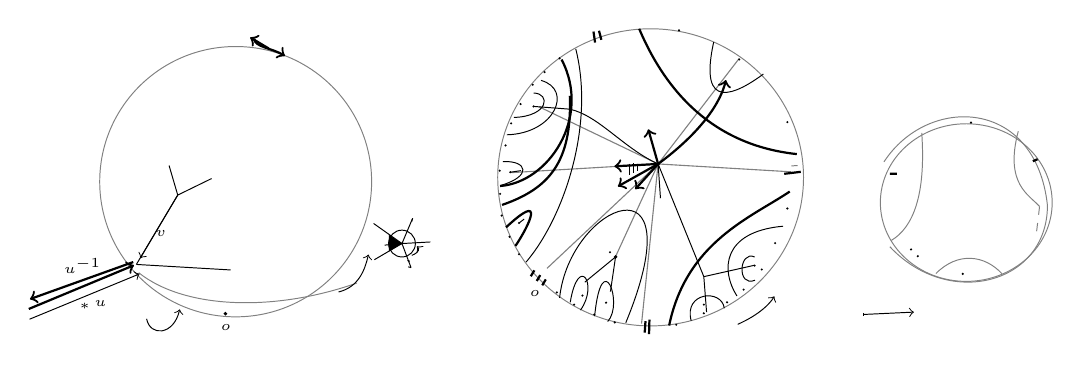
\begin{tikzpicture}[x=.005cm,y=-.005cm,every node/.style={font=\tiny,inner sep=1pt},line width=.35pt]
\draw[gray] (670,640) ellipse(345 and 343);
\draw[gray] (424,871)..controls(542,965)and(772,970)..(978,897);\draw[->,thick] (717,277)..controls(718,299)and(763,301)..(795,321);\draw[->,thick] (754,302)--(707,274);
\draw (418,850)--(523,674)--(501,599) (523,674)--(609,632) (418,850)--(657,864);\draw[->] (523,674)--(428,834);
\draw[->,thick] (410,844)--(148,938);\draw[->,thick] (145,963)--(412,852);\draw[->] (147,989)--(426,874);
\node at (282,853) {$u^{-1}$};\node at (327,950) {$u$};\node at (287,955) {$*$};\node at (480,771) {$v$};
\fill (644,975) circle(5);\node at (645,1011) {$o$};\draw[->] (444,988)..controls(453,1034)and(513,1030)..(528,964);
\draw (1092,797) circle(34);\draw (1092,797)--(1020,746) (1092,797)--(1119,733) (1092,797)--(1164,793) (1092,797)--(1115,858) (1092,797)--(1022,838);\fill (1092,797)--(1059,775)--(1059,817)--cycle;\draw[->] (1117,827)..controls(1139,818)and(1135,809)..(1130,804);\draw[->] (931,920)..controls(983,907)and(998,863)..(1007,825);
\draw (1092,797)--(1048,801) (1119,733)--(1117,741) (1112,842)--(1106,840) (1115,858)--(1108,856);
\draw[gray] (1723,629) ellipse(388 and 377);
\draw[gray,thin] (1742,595)--(1440,450) (1742,595)--(1370,617) (1742,595)--(1460,860) (1742,595)--(1635,828) (1742,595)--(1700,1000) (1742,595)--(2080,615) (1742,595)--(1948,327); \foreach \x/\y in {1345/726,1341/671,1340/612,1355/548,1369/492,1393/443,1424/394,1454/362,1492/327,1795/256,1948/330,2070/489,2070/708,2039/796,2005/863,1959/914,1917/946,1788/1003,1632/997,1580/977,1529/952,1485/921,1437/887,1389/824,1365/780}{\fill (\x,\y) circle(3);} \draw[thick] (1578,259)--(1582,287) (1592,257)--(1598,280) (2062,620)--(2104,615) (1710,994)--(1708,1023) (1720,990)--(1719,1027) (1428,865)--(1419,880) (1443,877)--(1434,892) (1457,888)--(1448,903); \draw[gray] (2080,600)--(2096,599); \node at (1429,925) {$o$}; \draw (1426,415)..controls(1470,416)and(1465,474)..(1376,477); \draw (1445,383)..controls(1527,406)and(1480,518)..(1358,521); \draw[thick] (1497,330)..controls(1574,477)and(1464,642)..(1341,651); \draw (1533,303)..controls(1582,497)and(1503,731)..(1407,844); \draw[thick] (1518,422)..controls(1524,592)and(1464,658)..(1346,699); \draw (1348,589)..controls(1410,586)and(1424,626)..(1341,650); \draw (1367,616)--(1394,612) (1389,745)--(1402,735); \draw[thick] (1356,756)..controls(1458,661)and(1415,751)..(1380,803); \draw (1426,449)--(1518,456)..controls(1591,472)and(1654,555)..(1742,595); \draw[thick] (1694,252)..controls(1760,408)and(1879,547)..(2094,570); \draw[thick,->] (1742,595)..controls(1853,513)and(1901,438)..(1914,382); \draw (1883,286)..controls(1843,467)and(1941,417)..(2009,367); \draw (1742,595)--(1858,881)--(1865,971) (1858,881)--(1987,852); \draw[thick] (1770,1005)..controls(1814,792)and(1980,730)..(2076,665); \draw (1660,998)..controls(1840,560)and(1517,697)..(1492,935); \draw (1519,946)..controls(1540,821)and(1592,900)..(1545,966); \draw (1581,981)..controls(1599,798)and(1656,950)..(1614,995); \fill (1634,831) circle(5);\draw (1634,831)--(1621,919) (1634,831)--(1556,895); \draw (1826,993)..controls(1806,920)and(1903,911)..(1910,961); \draw (2059,753)..controls(1903,767)and(1901,866)..(1942,930); \draw (1987,831)..controls(1947,813)and(1941,910)..(1988,890); \draw[->] (1944,1002)..controls(2000,977)and(2026,949)..(2037,931); \foreach \x/\y in {1426/449,1367/616,1389/745,1620/819,1858/952,1858/974,1987/853}{\fill (\x,\y) circle(3);} \draw[thick,->] (1742,595)--(1717,507);\draw[thick,->] (1742,595)--(1631,601);\draw[thick,->] (1742,595)--(1640,652);\draw[thick,->] (1742,595)--(1684,659);\draw (1742,595)--(1748,682);\fill (1742,595) circle(5);\draw (1670,594)--(1670,622) (1680,593)--(1680,618) (1690,594)--(1690,614); \fill (1550,929) circle(3) (1610,947) circle(3);
\draw[gray] (2524,693) ellipse(218 and 200);\draw[gray] (2315,590)..controls(2425,420)and(2700,425)..(2730,700)..controls(2730,900)and(2480,965)..(2330,805) (2411,516)..controls(2422,674)and(2389,756)..(2334,789) (2656,512)..controls(2620,647)and(2685,674)..(2710,703) (2447,873)..controls(2503,817)and(2571,826)..(2615,874); \foreach \x/\y in {2536/490,2384/812,2401/829,2515/874}{\fill (\x,\y) circle(3);}\draw[gray,dashed] (2710,703)--(2701,779); \draw[->] (2262,977)--(2391,971);\draw (2263,973)--(2263,980); \draw[thick] (2330,620)--(2348,620) (2693,588)--(2705,583);
\end{tikzpicture}}

\par\noindent\uline{NB} Alors l'ens. des arêtes issues d'un sommet quelq. est canoniq$^{t}$ \uline{ordonné}\par

\figure{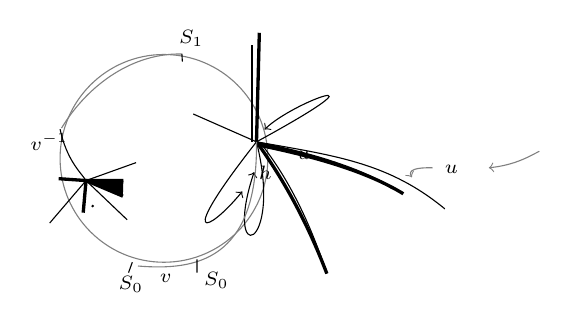
\begin{tikzpicture}[x=.006cm,y=-.006cm,every node/.style={font=\scriptsize,inner sep=1pt}]
\draw[gray] (365,350) ellipse(220 and 220);
\draw[gray] (148,286)..controls(205,192)and(301,126)..(404,129);
\draw (145,288)..controls(159,354)and(189,380)..(200,397);
\fill (200,397) circle(4) (561,315) circle(4);
\fill (200,397)--(279,397)--(278,430)--cycle;
\draw[very thick] (200,397)--(142,393) (200,397)--(279,397) (200,397)--(278,430) (200,397)--(194,465);
\draw (200,397)--(306,359) (200,397)--(287,480) (200,397)--(123,487);\fill (214,451) circle(3);
\draw (561,315)--(427,256);
\draw[very thick] (561,315)--(567,84);
\draw[thick] (551,315)--(551,110);
\draw (561,315)..controls(733,345)and(842,360)..(960,457);
\draw[very thick] (566,322)..controls(680,345)and(794,377)..(872,425);
\draw[thick] (565,317)..controls(680,340)and(785,373)..(850,414);
\draw[very thick] (561,315)..controls(624,402)and(672,495)..(710,594);
\draw (570,318)..controls(637,403)and(680,503)..(710,594);
\draw[->] (561,315)..controls(862,151)and(639,229)..(578,289);
\draw[->] (561,315)..controls(387,536)and(457,510)..(531,420);
\draw[->] (561,315)..controls(619,548)and(488,582)..(556,379);
\draw[gray] (561,315)..controls(564,567)and(432,588)..(310,578);
\draw (403,129)--(404,145) (298,570)--(290,592) (435,564)--(435,592);
\node at (423,96) {$S_1$};\node at (122,315) {$v^{-1}$};\node at (295,617) {$S_0$};\node at (369,604) {$v$};\node at (476,608) {$S_0$};\node at (661,343) {$u$};\node at (580,380) {$h$};\node at (974,374) {$\unsure{u}$};\draw[gray,->] (934,370)..controls(900,369)and(881,374)..(890,390);
\draw[gray,<-] (1053,370)..controls(1110,364)and(1140,345)..(1160,335);
\end{tikzpicture}}

La cat. des ``\deleted{\unsure{mots}}\inserted{types} de mots'' de long. $n$ \unsure{équivaut|équiv.-t} \unsure{à|:} la cat. \unsure{isotypique|isotopique} des systèmes formés d'un disque $D$ \inserted{en général orienté} d'un ``découpage par cordes'' de ce disque, avec au moins un sommet sur chaque arête découpée sur $\dot D$ par les extrémités des cordes,
\[
(D,\omega,\deleted{\unsure{K|S_0}},\deleted{\unsure{S}},K,S_0)
\]
$D$ le disque top.\par
$\omega$ une orientation de $D$\par
$K\subset D$ le 1-complexe top. (\unsure{réunion} top. de segments) des cordes du découpage\par
$S_0\in S$ \deleted{\unsure{est la composante} \unsure{de} \unsure{$\pi_0$|l'origine} $(\dot D\unsure{\setminus}K\cap\dot D)$}\par
\noindent\begin{tabular}{@{}ll@{}}
$S\subset\dot D$, & soit $R_0$ l'unique comp. connexe de\\
\unsure{et|de} $S\ne\varnothing$ & $D\setminus K$ contenant $S_0$
\end{tabular}

\[
\uline{\text{ordre réduit}}=\sum_{\alpha\in\pi_0(\dot D\setminus K\cap\dot D)}(\operatorname{Card}(\alpha\cap S)-1)
\]
\[
(\deleted{\text{\unsure{pour|ou}}\ \unsure{\alpha\in\pi_0}}\ \alpha\subset R_0)
\]
\margin{$v\,u^{-1}u$\par $u\,v\cdot u^{-1}$}

\noindent\begin{minipage}[t]{.39\linewidth}
Type de mot \uline{trivial} : ordre réduit $=0$\par
\uline{Type de mot totalitaire} : $K=\varnothing$\par
(\unsure{non|i.e.} trivial)
\end{minipage}\hfill\begin{minipage}[t]{.02\linewidth}\figure{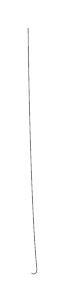
\begin{tikzpicture}[x=.014cm,y=-.014cm]\draw[gray,line width=.3pt] (1124,1921) .. controls (1125,2010) and (1128,2100) .. (1132,2140) .. controls (1132,2144) and (1129,2145) .. (1127,2143);\end{tikzpicture}}\end{minipage}\hfill\begin{minipage}[t]{.56\linewidth}
\[
\operatorname{Card}S=n\quad(\ne0)\qquad\text{donc }S\ne\varnothing
\]
\[
\deleted{\unsure{S\cap S_0\ne\varnothing}}\quad
\forall\alpha\in\pi_0(\dot D\setminus K\cap\dot D)
\left\{\begin{array}{l}
S\cap\alpha\ne\varnothing\\
\operatorname{Card}S\cap\alpha=1\quad\text{si }\alpha\not\subset R_0
\end{array}\right.
\]
Type de mot trivial,\par
si $\unsure{2}\ \operatorname{Card}S\cap\alpha$
\end{minipage}

\par\noindent{\ttfamily
/*JOB=CRAY1,ACCT=*********,ALL=\unsure{M06|MO6}\\
// JOB MSGLEVEL=(1,1),MSGCLASS=A\\
// EXEC CSSBATCH\\
//CRAYIN DD *\par}
\par\noindent{\ttfamily\unsure{J0202CNU|JO202CNU}}\par
\margin{2}

\scanpage{4}
\figure{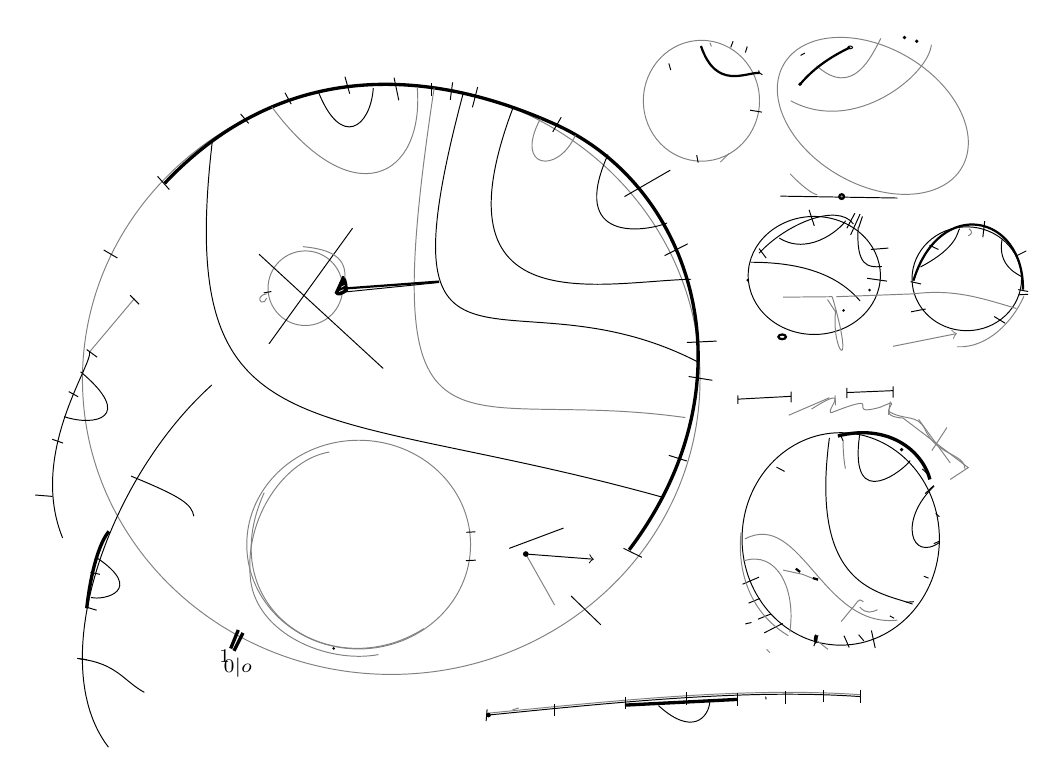
\begin{tikzpicture}[x=.006cm,y=-.006cm,line width=.35pt,every node/.style={font=\scriptsize,inner sep=1pt}]
\draw[gray] (802,865) ellipse(654 and 625);
\draw[very thick] (322,450)..controls(549,209)and(846,186)..(1156,328)..controls(1443,462)and(1574,872)..(1306,1226);
\draw (423,361)..controls(344,1037)and(630,907)..(1374,1114);
\draw[gray] (549,288)..controls(721,520)and(873,438)..(857,246);
\draw (648,257)..controls(696,377)and(758,332)..(764,248);
\draw[gray] (893,247)..controls(763,1108)and(930,876)..(1425,946);
\draw (955,257)..controls(768,960)and(1049,619)..(1453,829);
\draw (1061,287)..controls(885,750)and(1243,658)..(1437,653);
\draw[gray] (1118,313)..controls(1061,419)and(1155,432)..(1192,348); \draw (1261,389)..controls(1177,576)and(1338,553)..(1386,534);
\draw[gray] (163,807)--(258,694);
\foreach \x/\y/\a/\b in {307/435/332/463,193/591/222/608,157/802/179/818,249/687/268/706,483/303/500/323,577/258/590/282,704/224/714/260,808/226/818/274,888/237/888/265,932/236/927/273,985/246/974/289,1162/310/1144/341,1296/478/1393/422,1381/603/1430/578,1428/787/1491/784,1432/859/1482/867,1390/1026/1428/1038,1294/1223/1333/1242,1183/1324/1246/1385}{\draw (\x,\y)--(\a,\b);}
\draw[very thick] (478,1396)--(462,1435) (488,1402)--(469,1440);\node at (477,1475) {$\unsure{0|o}$};\node at (449,1452) {$1$};
\draw[gray] (733,1215) ellipse(237 and 221);\draw[gray] (533,1105)..controls(420,1352)and(677,1516)..(871,1393); \draw[gray] (671,1019)..controls(578,1034)and(489,1157)..(504,1290)..controls(518,1404)and(666,1468)..(775,1448);\draw (961,1189)--(980,1188) (960,1249)--(981,1248);\fill (680,1435) circle(3);
\draw[gray] (620,672) circle(79);\draw (522,600)--(785,842) (543,790)--(720,545);\draw[thick] (698,673)--(903,658);\draw (704,680)--(902,660)--(903,658);\fill (682,682)..controls(687,671)and(696,652)..(698,646)..controls(704,643)and(710,657)..(710,678)..controls(700,687)and(687,692)..(682,682)--cycle;\draw[white,line width=.25pt] (692,679)--(701,675) (696,670)--(703,666);\draw[gray] (615,584)..controls(680,590)and(706,610)..(704,650);\draw (532,682)--(548,679);
\draw[gray] (538,684)..controls(523,686)and(520,697)..(527,701)..controls(532,704)and(536,699)..(538,693);
\draw[gray] (1087,1235)--(1148,1343);\draw[->] (1087,1235)--(1231,1246);\draw (1052,1223)--(1167,1180);\fill (1087,1235) circle(6);
\draw (106,1201)..controls(33,1022)and(171,832)..(163,807);
\draw (144,849)..controls(260,946)and(175,966)..(109,944);\draw (119,891)--(139,902) (84,992)--(107,1000) (48,1110)--(85,1113);
\draw (203,1644)..controls(66,1466)and(201,1076)..(422,877);
\draw[very thick] (157,1350)..controls(166,1270)and(184,1211)..(204,1187);
\draw (177,1242)..controls(282,1312)and(194,1334)..(166,1327);
\draw (251,1070)..controls(358,1114)and(379,1129)..(384,1155);
\draw (142,1457)..controls(221,1467)and(234,1503)..(279,1528);
\draw (137,1456)--(158,1459) (155,1347)--(178,1354) (165,1274)--(185,1278);
\draw[gray] (1459,275) ellipse(123 and 128);\draw[thick] (1458,159)..controls(1490,254)and(1554,214)..(1582,216); \draw[gray] (1477,152)--(1480,160) (1499,405)--(1518,386);\draw (1580,211)--(1582,216)--(1588,220);
\foreach \x/\y/\a/\b in {1390/196/1394/210,1526/149/1521/162,1556/160/1552/173,1562/295/1587/299,1449/390/1452/406}{\draw (\x,\y)--(\a,\b);}
\draw[gray,rotate around={-30:(1822,307)}] (1822,307) ellipse(218 and 145);
\draw[gray] (1703,201)..controls(1781,271)and(1820,178)..(1839,143) (1648,275)..controls(1784,349)and(1941,219)..(1946,156);
\foreach \x/\y in {1668/240,1889/141,1915/149}{\fill (\x,\y) circle(4);}\draw[fill=white,thick] (1756,478) circle(5);
\draw[fill=white] (1774,162) ellipse(5 and 3);\draw (1626,477)--(1874,481); \draw[thick] (1668,240)..controls(1700,202)and(1740,178)..(1774,162);\draw (1669,179)--(1678,174);\draw[gray] (1647,430)..controls(1667,451)and(1692,472)..(1704,474);
\draw (1698,645) ellipse(140 and 125);\draw (1581,598)..controls(1638,536)and(1747,490)..(1781,536);\draw (1624,566)..controls(1693,608)and(1764,535)..(1764,529);\draw (1563,617)..controls(1673,617)and(1748,644)..(1795,699);\draw (1791,543)..controls(1786,625)and(1811,629)..(1841,626);
\foreach \x/\y/\a/\b in {1581/588/1596/608,1687/506/1698/540,1784/513/1767/545,1795/515/1775/559,1800/520/1792/544,1818/590/1855/587,1810/651/1852/657}{\draw (\x,\y)--(\a,\b);}
\draw[fill=white,thick] (1630,775) ellipse(8 and 5);
\fill (1557,655) circle(3) (1760,719) circle(3) (1815,676) circle(3);\draw[gray] (1736,690)..controls(1787,862)and(1734,810)..(1743,722)--(1726,696);
\draw[gray] (1632,691)--(1736,690) (1745,690)--(1908,684);
\draw (2021,652) ellipse(116 and 110);\draw[thick] (1908,656)..controls(1963,476)and(2142,515)..(2140,675);
\draw (1923,627)..controls(2006,583)and(2000,551)..(2006,546) (2096,567)..controls(2084,627)and(2133,644)..(2138,648);
\draw[gray] (2026,546)..controls(2033,552)and(2033,557)..(2024,561);
\draw[gray] (1908,684)..controls(1993,673)and(2053,693)..(2126,715);\draw[gray,->] (1865,795)--(2000,768);\draw[gray] (2000,796)..controls(2066,800)and(2120,740)..(2142,689);
\foreach \x/\y/\a/\b in {1902/658/1924/663,1942/581/1961/590,2059/530/2055/564,2125/604/2147/593,2130/675/2151/679,2130/686/2151/685,1903/722/1934/716,2079/732/2102/746}{\draw (\x,\y)--(\a,\b);}
\draw (1536,907)--(1649,901) (1536,899)--(1536,917) (1649,891)--(1649,914) (1767,893)--(1864,889) (1767,883)--(1767,905) (1865,880)--(1865,904);
\draw[gray] (1692,928)..controls(1792,865)and(1704,951)..(1741,933)..controls(1855,889)and(1755,947)..(1838,924)..controls(1900,896)and(1814,943)..(1886,947)--(2024,1052)--(1986,1077);
\draw (1754,1203) ellipse(209 and 225);\draw[very thick] (1748,985)..controls(1853,958)and(1926,1014)..(1943,1077);
\draw (1730,989)..controls(1687,1309)and(1837,1315)..(1906,1341);
\draw[gray] (1759,995)..controls(1759,1018)and(1761,1040)..(1764,1054);
\draw (1794,983)..controls(1770,1155)and(1893,1052)..(1901,1037);
\draw (1952,1091)..controls(1875,1164)and(1903,1253)..(1964,1210);
\draw[gray] (1551,1203)..controls(1670,1141)and(1715,1393)..(1874,1375) (1547,1250)..controls(1620,1225)and(1660,1312)..(1646,1401);
\foreach \x/\y/\a/\b in {1618/1051/1635/1060,1752/980/1759/995,1927/1055/1942/1069,1546/1299/1581/1284,1559/1339/1583/1329,1579/1373/1606/1362,1592/1402/1631/1382,1706/1407/1697/1430,1761/1408/1772/1433,1792/1406/1803/1419,1819/1397/1827/1434}{\draw (\x,\y)--(\a,\b);}
\draw[gray] (1755,1378)--(1784,1343)..controls(1795,1327)and(1796,1333)..(1802,1336);
\draw[gray] (1794,1347)..controls(1808,1363)and(1821,1358)..(1832,1353);
\fill (1883,1014) circle(4); \draw[gray] (1644,941)--(1730,904) (1742,899)--(1743,920) (1859,912)--(1855,940);
\draw[gray] (1856,933)..controls(1889,953)and(1916,938)..(1932,970)..controls(1956,1026)and(2016,1022)..(2017,1054);
\draw[gray] (1919,950)--(1986,1042) (1979,967)--(1947,1016);
\draw[gray] (1543,1189)..controls(1535,1259)and(1554,1355)..(1643,1408);
\draw[gray] (1632,1269)--(1673,1278)--(1706,1291);\draw[thick] (1659,1266)--(1668,1273) (1695,1286)--(1706,1289);
\draw (1933,1107)--(1951,1090) (1955,1149)--(1963,1156) (1951,1213)--(1963,1208) (1930,1282)--(1940,1286) (1892,1337)--(1909,1336) (1858,1366)--(1867,1371);
\draw[gray] (1706,1420)--(1727,1437) (1597,1437)--(1604,1444);\draw (1552,1383)--(1565,1380);\fill (1701,1415) ellipse(4 and 10);
\draw[gray] (1008,1572)..controls(1282,1545)and(1554,1516)..(1796,1533);\draw (1008,1576)..controls(1282,1549)and(1554,1520)..(1796,1537);\draw[very thick] (1297,1555)--(1534,1543);\fill (1008,1576) circle(5);\draw (1005,1564)--(1003,1589) (1595,1537)--(1596,1543);\draw[gray] (1059,1565)--(1072,1561);
\foreach \x/\y in {1147/1566,1299/1551,1427/1541,1535/1544,1637/1540,1717/1536,1796/1537}{\draw (\x,\y-14)--(\x,\y+13);}\draw (1368,1556)..controls(1440,1622)and(1475,1581)..(1477,1546);
\end{tikzpicture}}

Structure : Graphe segment, avec inv. \inserted{$\sigma$} sur l'ens. des arêtes

\unsure{.} \uline{admissible} se définit par réc sur le nb $n$ d'arêtes (ordre du graphe)
\[
\begin{array}{l|l}
\Gamma\ \text{admissible}&\sigma=\mathrm{id}\\
\text{d'ordre }n\geq1&\text{ou }\exists\ \text{orbite }\inserted{\unsure{\varepsilon|\xi}}\text{ de }\sigma\text{ formée de deux arêtes consécutives,}
\end{array}
\]
\uline{et} le graphe \inserted{$\Gamma'$} déduit de $\Gamma$ par contraction en 1 point de l'une des \deleted{\unsure{deux}} arêtes $\in\unsure{\varepsilon|\xi}$, \deleted{\unsure{est}} muni de l'involution $\sigma'$ déduite de $\sigma$, est admissible

\margin{Tout graphe inv. d'ordre 0 est adm. (ceux d'ordre 1 aussi)}

\figure{\begin{tikzpicture}[x=.006cm,y=-.006cm,line width=.4pt]
\draw (283,2508)..controls(533,2196)and(870,2292)..(1093,2415);
\draw (416,2384)..controls(446,2436)and(451,2474)..(444,2553);
\draw (545,2328)..controls(574,2472)and(706,2460)..(740,2304);
\draw (881,2332)..controls(853,2392)and(851,2460)..(848,2491);
\fill (478,2353) circle(4) (835,2312) circle(4);
\draw[fill=white] (642,2306) ellipse(5 and 3); \fill (1081,2409) circle(2);
\draw[gray] (1373,2540) ellipse(315 and 290);
\draw[gray] (1073,2533)..controls(1008,2771)and(1169,2792)..(1251,2820) (1688,2516)..controls(1704,2737)and(1577,2791)..(1384,2835);
\draw (1248,2813)..controls(1232,2747)and(1368,2735)..(1370,2838);
\draw[gray] (1200,2793)--(1226,2753) (1414,2798)--(1423,2878);
\fill (1203,2788) circle(2.5) (1316,2829) circle(5) (1420,2831) circle(4);\draw[very thick] (1273,2811)--(1272,2821) (1291,2820)--(1290,2830) (1337,2827)--(1339,2838);
\draw (1884,2393) ellipse(93 and 91);
\draw (1792,2434)..controls(1745,2478)and(1713,2491)..(1689,2504) (1858,2308)--(1829,2234) (1924,2307)--(1955,2235) (1952,2451)--(1997,2506);
\draw (1798,2329)--(1813,2341) (1962,2330)--(1951,2340) (1876,2474)--(1873,2494);
\fill (2010,2538) circle(2); \draw[gray] (1061,2574)..controls(1083,2489)and(1109,2482)..(1061,2581);\draw[gray] (1800,2350)..controls(1779,2391)and(1789,2446)..(1841,2460) (1907,2302)..controls(1958,2315)and(1989,2370)..(1976,2433);
\end{tikzpicture}}
\margin{3}

\scanpage{5}
% H00: heading; the dark author page number is at the head.
\uline{Arbres plans.}\hfill\mspage{1}

% L01
Rappelons qu'un \uline{arbre}\inserted{(comb)} est un graphe (comb.)
% L02
1-connexe (ce qui implique que c'est un graphe
% L03
strict, i.e. sans bords fermés, et pas deux \deleted{\unsure{pts|points}}\inserted{sommets}
% L04: the doubt concerns the raised s-like glyph and its attachment within arête.
distincts joints \unsure{au|en} plus une arête\unsure{\inserted{s}}). On peut donc
% L05
considérer la structure donnée par $(S,A)$,
% L06
$S$ ens des sommets, $A\subset\mathcal P_2(S)$. \deleted{$\unsure{A}$} L'ens $S$ est $\ne\varnothing$,
% L07
et $A\deleted{\ne}=\varnothing\iff\operatorname{card}S=1$ (arbre \uline{ponctuel}).

% L08
On appelle \uline{arbre plan} un arbre muni d'une
% L09
classe de plongements\inserted{(de sa réal top)} dans une surface
% L10
(deux plongements étant identifiés $|\Gamma|\hookrightarrow X$
% L11
$|\Gamma|\hookrightarrow X'$ \unsure{s'il|; il} existe des voisinages\inserted{$U,U'$} de $|\Gamma|$ ds $X,X'$
% L12
et un homéo. $U\simeq U'$ induisant l'identité sur $|\Gamma|$).
% L13
Les \inserted{classes de} plongement (vu que $|\Gamma|$ est 1-connexe et
% L14
admet un voisinage ouvert 1-connexe $U$ dans $X$,
% L15
-- d'où $U\simeq\unsure{\mathbb R|\mathbb R^2}$ --) s'identifient aux \uline{bicircularisations}
% L16
de $\Gamma$, i.e. les \deleted{applications} \unsure{paires} $(\varepsilon,\unsure{c|\varphi|f})$, $\varepsilon$ un
% L17
ens à 2 éléments, \deleted{$\unsure{c|\varepsilon}$} et $c:\varepsilon\longrightarrow\operatorname{circ}(\Gamma)$
% L18
$c$ compatible aux ``passages à l'opposé''. Ici $\operatorname{circ}(\Gamma)$
% L19
est l'ens des \uline{circularisations} de $\Gamma$, i.e.
% L20
des systèmes d'ordres circulaires sur les
% L21
$A_s$ (où pour $\forall s\in S$, $A_s$ est l'ens des arêtes incidentes
% L22
à $s$). Une \inserted{classe de} plongement de $|\Gamma|$ dans une surface
% L23
\uline{orientée} correspond à une circularisation de
% L24
$\Gamma$; ça ne dépend que de \unsure{l'ens|l'une|la} famille des
% L25
$A_s$ $(s\in S)$ tels que $\operatorname{card}A_s\geq3$. Donc si les sommets
% L26
de $\Gamma$ sont d'ordre $\leq1$, il y en a \unsure{un|une} et un seul
% Thin grey foliation in another hand.
\margin{4}

\scanpage{6}
{\ttfamily\tiny
\begin{tabular}{l}
STMT NO. MESSAGE\\
-\\
\quad 4\quad IEF653I SUBSTITUTION JCL - PGM=CRBATCH,REGION=100K,PARM=\\
\$HASP373 STARTED - INIT 10 - CLASS Q - SYS E333\\
IEF236I ALLOC. FOR PREDONTA CSSBATCH\\
IEF237I 581\quad ALLOCATED TO STEPLIB\\
IEF237I 2C9\quad ALLOCATED TO SYS00036\\
IEF237I VIO\quad ALLOCATED TO SYSUT1\\
IEF237I JES2 ALLOCATED TO SYSUDUMP\\
IEF237I 59F\quad ALLOCATED TO CRJIF\\
IEF237I JES2 ALLOCATED TO SYSIN\\
CSS2090 - JOB INPUT FILE TEMPORARILY FULL - PLEASE TRYAGAIN LATER\\
IEF142I PREDONTA CSSBATCH - STEP WAS EXECUTED - COND CODE 0000\\
IEF285I\quad CISI.PROD.CSSBATCH.V1.YY01\hspace{2cm}KEPT\\
IEF285I\quad VOL SER NOS= MVS104.\\
IEF285I\quad SYSCTLG.VSAC015\hspace{3cm}KEPT\\
IEF285I\quad VOL SER NOS= SAC015.\\
IEF285I\quad SYS82139.T163912.RA000.PREDONTA.SYSUT1\quad DELETED\\
IEF285I\quad JES2.JOB01125.\unsure{SO0102|S00102}\hspace{2cm}SYSOUT\\
IEF285I\quad SYS1.CR.JIF\hspace{3.5cm}KEPT\\
IEF285I\quad VOL SER NOS= CRAY11.\\
IEF285I\quad JES2.JOB01125.SI0101\hspace{2cm}SYSIN\\
IEF373I STEP /CSSBATCH/ START 82139.1639\\
IEF374I STEP /CSSBATCH/ STOP\quad 82139.1639 CPU\quad 0MIN 00.05SEC SRB\quad 0MIN 00.00SEC VIRT\quad 20K SYS\quad 184K\\
IEF375I JOB /PREDONTA/ START 82139.1639\\
IEF376I JOB /PREDONTA/ STOP\quad 82139.1639 CPU\quad 0MIN 00.05SEC SRB\quad 0MIN 00.00SEC
\end{tabular}}
\margin{5}

\scanpage{8}
\mspage{2}
On a une application bijective.
\[
\vec A\overset{\mathrm{rd}}{\simeq}A_{\unsure{*|\leftarrow|+}}(C)\quad\text{ens des arêtes de }C
\]
\[
\vec a\longmapsto\text{``rive \deleted{\unsure{gauche}}\inserted{droite} de $\unsure{-|\vec a}$''}
\]
et chaque arête de $C$ est orientée de façon naturelle via cette application. Donc l'ens. des \uline{arcs} $\vec A(C)$ s'identifie :
\[
A(C)\times\{\pm1\}\simeq\vec A\times\{\pm1\},
\]
et l'application $\sigma_0^C$ (passage à \unsure{l'autre|l'arête} opposée) s'identifie : $\deleted{\unsure{\sigma}}\unsure{\sigma_\Gamma|\mathrm{id}|\sigma_0}\times\tau$, $\tau$ la transposition de $\pm1$. Reste : définir $\sigma_1^C$, on le définit séparément sur
\[
\underbrace{\vec A\times\{+1\}}_{=\uline{\mathrm{rg}(\vec A)}}=\vec A(C)_+
\]
et sur
\[
\underbrace{\vec A\times\{-1\}}_{\mathrm{rd}(\vec A)}=\vec A(C)_-.
\]
On a :
\margin{\uline{NB} $\vec A(C)_+$ est une \uline{orientation} des contours}
\figure{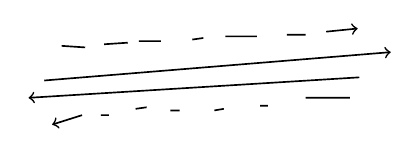
\begin{tikzpicture}[x=.02cm,y=-.02cm,line width=.6pt]
\draw[->] (115,705)--(335,687);
\draw[->] (315,703)--(105,716);
\draw (126,683)--(141,684) (153,682)--(168,681) (175,680)--(189,680) (209,679)--(216,678) (230,677)--(250,677) (269,676)--(281,676);
\draw[->] (294,674)--(314,672);
\draw[<-] (120,733)--(139,727);
\draw (151,727)--(156,727) (173,723)--(180,722) (195,724)--(201,724) (223,724)--(229,723) (252,721)--(257,721) (281,716)--(309,716);
\end{tikzpicture}}
\figure{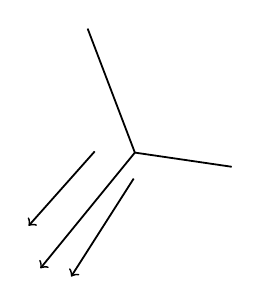
\begin{tikzpicture}[x=.015cm,y=-.015cm,line width=.65pt]
\draw (145,969)--(185,1074)--(267,1086);
\draw[->] (185,1074)--(105,1172);
\draw[->] (151,1073)--(95,1136);
\draw[->] (184,1096)--(131,1179);
\end{tikzpicture}}
\margin{$A$}
\figure{\begin{tikzpicture}
\node[inner sep=3pt] (f) {$\displaystyle
\left\{\begin{aligned}
\sigma_1^C(\mathrm r\deleted{\unsure{\mathrm g}}\mathrm d(\vec a))&=\deleted{\unsure{\mathrm{rd}}}\mathrm{rg}(\rho_\Gamma^{-1}(\vec a))=\sigma_0^C\mathrm{rd}(\rho_\Gamma(\vec a))\\
\sigma_1(\mathrm r\deleted{\unsure{\mathrm d}}\mathrm g(\vec a))&=\mathrm r\deleted{\unsure{\mathrm g}}\mathrm d(\rho_\Gamma^{\deleted{\unsure{-1}}}(\vec a))\deleted{\unsure{=\sigma_0^C}}
\end{aligned}\right.$};
\draw ([xshift=3pt,yshift=7pt]f.north west)--([xshift=7pt,yshift=7pt]f.north east);
\draw[->] ([xshift=7pt,yshift=7pt]f.north east)--([xshift=3pt]f.east);
\draw ([xshift=3pt,yshift=-1pt]f.east)--([xshift=3pt,yshift=-5pt]f.south east);
\draw ([xshift=1pt,yshift=-5pt]f.south east)--([xshift=-6pt,yshift=-5pt]f.south west)--([xshift=-6pt,yshift=1pt]f.north west);
\end{tikzpicture}}
\[
\Longrightarrow\quad\cdot\quad
\deleted{\rho_s(\vec a)=}
\left\{\begin{aligned}
\rho_C(\mathrm{rd}\vec a)&=\mathrm{rd}(\rho_\Gamma^{\deleted{\unsure{-1}}}(\vec a))\\
\rho_C(\mathrm{rg}\vec a)&=\mathrm{rg}(\rho_\Gamma^{-1}\deleted{\unsure{\sigma_\Gamma}}\vec a))
\end{aligned}\right.
\]
\margin{\uline{NB} \inserted{La définition} des \uline{contours} \uline{orientés} $C$ ne dépend que de $\vec A$ muni de $\rho_\Gamma$ (à l'exclusion de $\sigma_0$)}

\unsure{Le} contour $C$ : \unsure{incidé} \unsure{sens} des \unsure{Aristyp.}

a) $C$ est orienté (``sens \unsure{direct|évident} autour de $\Gamma$'')
\deleted{\deleted{\unsure{C|le}} \deleted{\unsure{A|C}} $C'$ par ``juxtaposition'' i.e. chaque \inserted{(tient compte de $\unsure{o}$)} \unsure{arête|est} \unsure{est} \unsure{orientée}, soit la donnée d'une application \unsure{canonique}}
\[
\deleted{\vec A(C)'_+\subset\vec A(C),}
\]
\deleted{(``\unsure{plages} \unsure{topologiques}'') : la \unsure{unique} p.}
\[
\deleted{A(C)\longrightarrow\pm1}
\]
\deleted{\unsure{donnant} la valeur \unsure{$+1$ et $-1$} sur les deux \unsure{côtés}.}

\margin{i.e. on a ---\par
$\vec A=\vec A(C)_+\subset\vec A(C)$\par
ou\par
$\sigma_0\vec A=\vec A(C)_-\unsure{\sim\vec A|\simeq\vec A|\deleted{\sim\vec A}|\deleted{\simeq\vec A}}$\par
$\sigma_1\vec A=\vec A(C)_-\unsure{\sim\vec A|\simeq\vec A|\deleted{\sim\vec A}|\deleted{\simeq\vec A}}$}
Donc
\[
\left\{\begin{aligned}
\vec A(C)&\simeq\uline{\vec A(C)_+}\times\{\pm1\},\\
\sigma_0^C&\simeq\mathrm{id}\times\tau
\end{aligned}\right.
\]
La donnée de $\sigma_1^C$ revient à celle d'une permutation
\[
\rho_C^{\unsure{\bullet}}=\hookleftarrow\{\vec a\longrightarrow\sigma_1^C(\sigma_0^C(\vec a)))\quad\text{sur }\vec A
\]
b) On a une involution, sans pts fixes \inserted{$\sigma_{\unsure{0|\Gamma}}^C$} sur l'ens \deleted{\unsure{des}} des côtés de $\unsure{\Delta|C}$, qui s'identifie :
\[
\vec A=\vec A(C)_+.
\]
\margin{7}

\scanpage{10}
\mspage{2'}
Ces deux données pour le contour $C$ permettent de récupérer un graphe circularisé\unsure{s|,} $\Gamma$, ayant $\vec A$ comme ens des arêtes orientées, avec opérations $\sigma_A$, $\rho_S$ données ainsi :
\[
\left\{\begin{aligned}
\sigma_\Gamma&=\sigma_C\\
\rho_\Gamma&=\rho_C
\end{aligned}\right.
\]

\uline{En résumé} La catégorie des \inserted{$\underset{\cdot}{\unsure{c|C}}$}%
% Placement after des records horizontal position only; attachment remains unresolved.
 graphes combinatoires circularisés $\Gamma$ (sans sommet isolé) \inserted{$(\vec A\deleted{\unsure{_\Gamma}}(\Gamma),\rho_\Gamma,\sigma_\Gamma)$} est équivalente à celle des contours orientés, avec involution \inserted{\unsure{ss|s} pt fixe $\sigma_C$} sur l'ens des \uline{arêtes}, soit $C$ ($=A(C)$ ens des arêtes de $C$, $\rho_C$ rotation fondamentale de $C$, $\sigma_C$ involution sur $A(C)$). \deleted{\unsure{par} \inserted{\unsure{la|le|C}} \illegible{1}} \deleted{\unsure{p}} correspondance fondamentale \unsure{:|;}
\diagram{\begin{tikzcd}[row sep=large,column sep=large]
\vec A(\Gamma)&A(C)\arrow[l,"\sim"']\\
\sigma_\Gamma\arrow[r,leftrightarrow]&\unsure{\sigma_C|\rho_C}\\
\rho_{\unsure{\Gamma|\deleted{\Gamma}}}^{\unsure{r|\sigma|-1|\delta}}\sigma_\Gamma&\rho_C\arrow[l,*->]\\
\rho_\Gamma&\rho_C\sigma_C\arrow[l,*->]
\end{tikzcd}}
\margin{On appellera \unsure{cela|$C$ le} \uline{déploiement} du graphe plan donné}
\margin{$\rho_\Gamma^{\unsure{r|\sigma}}$ rotation-sommets pour la carte \unsure{actuel|actuelle} défini par $\Gamma$}

\figure{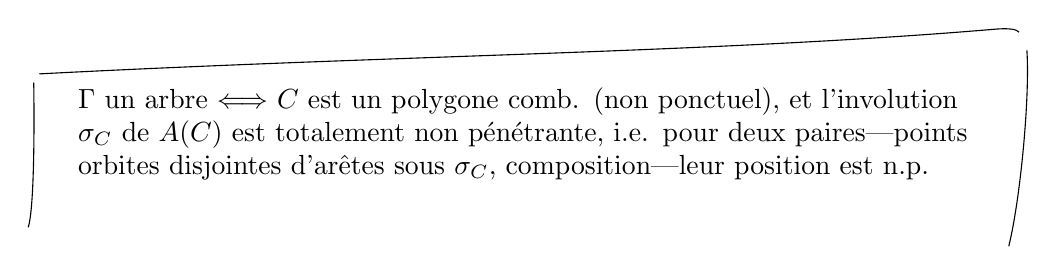
\begin{tikzpicture}[x=.01cm,y=-.01cm]\draw (238,1972) .. controls (700,1948) and (1100,1945) .. (1455,1915) .. controls (1470,1914) and (1480,1915) .. (1483,1919);\draw (231,1983) .. controls (232,2055) and (231,2145) .. (224,2167);\draw (1493,1942) .. controls (1497,2000) and (1485,2130) .. (1470,2191);\node[anchor=north west,align=left,text width=11.8cm] at (275,1977) {$\Gamma$ un arbre $\Longleftrightarrow$ $C$ est un polygone comb. (non ponctuel), et l'involution $\sigma_C$ de $A(C)$ est totalement non pénétrante, i.e. pour deux \deleted{\unsure{paires|points}} \inserted{orbites} disjointes d'arêtes sous $\sigma_C$, \unsure{composition|leur position} est n.p.};\end{tikzpicture}}
\margin{09}

\scanpage{11}
\mspage{3}
% Header: one upper and three lower physical text baselines, plus the arrow/sign band.
% The doubtful comma represents the detached curve before combinatoires; its physical attachment is open.
\diagram{\begin{tikzcd}[row sep=huge]
{\text{``Arbres plans''}\text{\rlap{\raisebox{1.8ex}{\inserted{(non ponctuels)}}}}\text{ (dans un plan pas néc. \deleted{orienté})}}\arrow[d,leftrightarrow,"\approx",to path={([xshift=-4cm]\tikztostart.south)--([xshift=-4cm]\tikztotarget.north)\tikztonodes}]\\
{\begin{gathered}\text{polygônes\unsure{,} combinatoires, avec \deleted{\unsure{involution|relation}} inv. sans}\\\text{pts fixes non pénétrante sur l'ens des}\\\text{\deleted{\unsure{sommets}}\inserted{\unsure{arêtes|côtés}.}}\end{gathered}}
\end{tikzcd}}
\par\noindent\rule{\linewidth}{.4pt}

% L01
Revenant au cas d'un graphe $\Gamma$ circularisé \inserted{général},
% L02
Topologiquement, le graphe top. $|\Gamma|$
% L03
se déduit de $|C|$ par \deleted{\unsure{les identifications}}
% L04
\unsure{un|i.e.} quotient par \unsure{la|C} relation d'%
% L05
équivalence suivante : on recolle
% L06
l'arête $a$ et l'autre $\unsure{\sigma_C a|\sigma_C^a}$, en \uline{renversant} les
% L07
orientations induites sur ces \unsure{arêtes|côtés}.

% L08
Dans le cas où $\Gamma$ est un
% L09
arbre, on peut interpréter
% L10
celui-ci \inserted{top.${}^{t}$} en considérant
% L11
$C$ comme le bord
% L12
d'un disque orienté $D$,
% L13
subdivisé en \unsure{arêtes|côtés}, et
% L14
en joignant les ``centres''
% L15
des \unsure{arêtes|côtés} qui se correspondent
% L16
par $\sigma_C$, de façon à ce que les seg-\linebreak
% L17
ments obtenus ne se rencontrent pas.

\figure{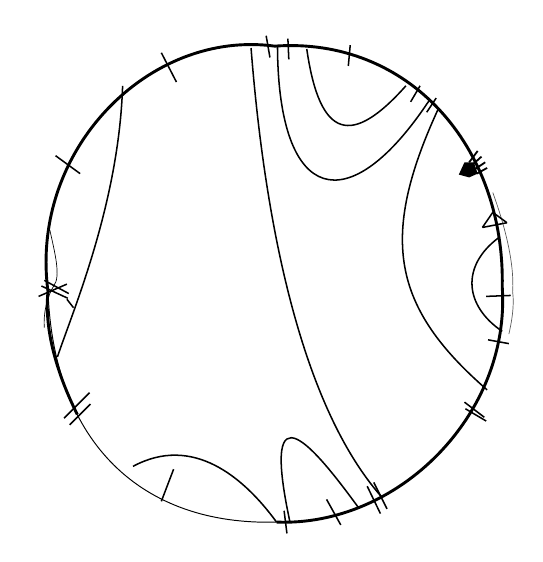
\begin{tikzpicture}[x=.012cm,y=-.012cm,line width=.55pt]
% F01 Thin continuous boundary, including thin lower-left arc
\draw[line width=.35pt] (95,1640).. controls (75,1490) and (202,1362)..(335,1380).. controls (476,1370) and (579,1485)..(576,1635).. controls (585,1770) and (466,1889)..(337,1884).. controls (194,1888) and (101,1800)..(95,1640);
% F02 Heavier retraced left, upper, right and lower-right boundary
\draw[line width=1.05pt] (126,1770).. controls (102,1722) and (91,1676)..(95,1640).. controls (75,1490) and (202,1362)..(335,1380).. controls (476,1370) and (579,1485)..(576,1635).. controls (585,1770) and (466,1889)..(337,1884);
% F03 Thin outer return beside heavy right rim; local ends approximate
\draw[line width=.25pt,black!65] (566,1535).. controls (579,1571) and (589,1610)..(587,1640).. controls (589,1655) and (586,1672)..(583,1685);
% F04 Interior curve1 close to left rim
\draw (174,1422).. controls (170,1547) and (121,1661)..(105,1709);
% F05 Interior curve2 long upper-to-lower-right span
\draw (310,1382).. controls (326,1586) and (368,1766)..(448,1857);
% F06 Interior curve3 larger upper-right nested cup
\draw (338,1381).. controls (339,1547) and (413,1567)..(499,1437);
% F07 Interior curve4 smaller upper-right cup
\draw (369,1383).. controls (383,1480) and (417,1486)..(474,1422);
% F08 Interior curve5 bowed left from right rim
\draw (508,1447).. controls (445,1584) and (460,1657)..(560,1744);
% F09 Interior curve6 small middle-right cup
\draw (572,1583).. controls (532,1613) and (536,1655)..(576,1682);
% F10 Interior curve7 low bottom-left arch
\draw (185,1825).. controls (248,1791) and (302,1836)..(337,1884);
% F11 Interior curve8 small upright bottom arch
\draw (351,1883).. controls (319,1733) and (378,1806)..(424,1869);
% F12 Single oblique crossing tick
\draw (215,1387)--(231,1418);
% F13 First short near-vertical top tick
\draw (326,1369)--(330,1392);
% F14 Second short near-vertical top tick
\draw (349,1372)--(350,1394);
% F15 Single near-vertical tick
\draw (415,1379)--(413,1401);
% F16 First tick crossing rim obliquely
\draw (479,1439)--(489,1422);
% F17 Second tick crossing rim obliquely
\draw (496,1450)--(506,1435);
% F18 Merged dark inner part of four-pronged hatch; no inferred four full crossings
\fill (530,1516)--(536,1503)--(546,1503)--(550,1515)--(541,1519)--cycle;
% F19 Visible outward prong, inner end merged into F18
\draw[line width=.65pt] (541,1503)--(550,1491);
% F20 Visible outward prong, inner end merged into F18
\draw[line width=.65pt] (543,1507)--(554,1497);
% F21 Visible outward prong, inner end merged into F18
\draw[line width=.65pt] (546,1511)--(558,1503);
% F22 Visible outward prong, inner end merged into F18
\draw[line width=.65pt] (549,1515)--(560,1509);
% F23 First edge of triangular mark
\draw (555,1572)--(581,1567);
% F24 Second edge of triangular mark
\draw (581,1567)--(566,1556);
% F25 Third edge closing triangular mark
\draw (566,1556)--(555,1572);
% F26 Transverse tick
\draw (559,1645)--(585,1644);
% F27 Transverse tick
\draw (561,1691)--(583,1695);
% F28 First trace of paired mark
\draw (536,1757)--(557,1773);
% F29 Second trace of paired mark
\draw (537,1764)--(559,1777);
% F30 First trace of paired mark
\draw (433,1846)--(447,1875);
% F31 Second trace of paired mark
\draw (440,1842)--(454,1870);
% F32 Single oblique bottom tick
\draw (390,1860)--(405,1887);
% F33 Near-vertical bottom tick
\draw (345,1872)--(348,1896);
% F34 Oblique tick on thin arc
\draw (228,1828)--(215,1862);
% F35 First close trace of paired mark
\draw (112,1774)--(139,1747);
% F36 Second close trace of paired mark
\draw (118,1781)--(140,1759);
% F37 First crossing stroke
\draw (85,1645)--(115,1632);
% F38 Second crossing stroke
\draw (88,1634)--(116,1647);
% F39 Third crossing stroke
\draw (91,1628)--(117,1642);
% F40 Detached short oblique fragment
\draw (115,1648)--(122,1657);
% F41 Single crossing tick
\draw (103,1496)--(129,1515);
% F42 Thin parallel returning trace beside heavy rim and hatch; ends approximate
\draw[line width=.25pt] (97,1575).. controls (102,1598) and (109,1624)..(101,1634).. controls (94,1645) and (90,1663)..(91,1678);
\end{tikzpicture}}

% L18
Les sommets de $\Gamma$ correspondent alors
% L19
aux régions découpées dans $D$, et les arêtes
% L20
orientées de $\Gamma$ aux frontières communes orientées,
% Thin grey other-hand foliation.
\margin{10}

\scanpage{12}
{\footnotesize\begin{tabular}{rlll}
\texttt{1}&\texttt{//PREDONTA}&\texttt{JOB '*********,00000000C','\hspace{4em}',}&\texttt{JOB 1125}\\
&\texttt{//}&\texttt{MSGLEVEL=(1,1)}&\\
\texttt{2}&\texttt{//}&\texttt{EXEC CSSBATCH}&\\
\texttt{3}&\texttt{XXCSSBATCH}&\texttt{PROC REG=100K,P=''}&\texttt{00010000}\\
\texttt{4}&\texttt{XXCSSBATCH}&\texttt{EXEC PGM=CRBATCH,REGION=\&REG,PARM=\&P}&\texttt{00020000}\\
\texttt{5}&\texttt{XXSTEPLIB}&\texttt{DD DSN=CISI.PROD.CSSBATCH.V1.YY01,DISP=SHR}&\texttt{00030003}\\
\texttt{6}&\texttt{XXSYSUT1}&\texttt{DD DSN=\&\&SYSUT1,UNIT=\unsure{SYSTSO|SYSTS0},SPACE=(TRK,30),DISP=(NEW,DELETE)}&\texttt{00031006}\\
\texttt{7}&\texttt{XXSYSUDUMP}&\texttt{DD SYSOUT=*}&\texttt{00040000}\\
\texttt{8}&\texttt{XXCRJIF}&\texttt{DD DSN=SYS1.CR.JIF,DISP=SHR}&\texttt{00050000}\\
\texttt{9}&\texttt{XXSYSIN}&\texttt{DD DDNAME=CRAYIN}&\texttt{00060000}\\
\texttt{10}&\texttt{//CRAYIN}&\texttt{DD *}&
\end{tabular}}
\margin{11}

\scanpage{13}
\mspage{3'}
\unsure{donc|dont|dans} le graphe $\Gamma$ exprime \unsure{la|le} façon dont les régions se raccordent suivant des frontières communes.

La catégorie des arbres plans \inserted{(pas néc. plus orientés)} est équiva\unsure{-}\linebreak
lente : la catégorie isotypique des disques \deleted{\unsure{orientés}} (pas néc. orientés \unsure{donc|de non|ou non}) munis d'un tel découpage. Le polygone combinatoire \deleted{\unsure{le contour|qui correspond}} \inserted{$\unsure{C}$}%
% The raised C-like curve touches the preceding decoupage descender; its identity and insertion attachment remain doubtful.
 est \uline{dual} de celui défini par les cordes du découpage sur le bord des disques, les sommets de $\Gamma$ correspondant à des paquets d'arêtes de ce contour (celles qui bordent une région déterminée du découpage \deleted{\unsure{du}} du disque).
\margin{12}
